\documentclass[a4paper, 12pt]{report}

% Packages
\usepackage{amsmath}
\usepackage{amssymb}
\usepackage[margin=1in]{geometry}
\usepackage{hyperref}
\usepackage{graphicx}
\usepackage{subcaption}
\usepackage{float}

%Indentation and spacing
\setlength{\parindent}{0pt}

\begin{document}


%%%%%% Chap - 0 %%%%%%

\section*{Chapter 1:    Introduction}

In today's world, there has been a rapid development in infrastructure, including buildings and bridges, to meet the needs of the 
people. Hence, the requirement for slender bridges is gaining importance to make it a sustainable construction by the optimal use 
of material. For spans greater than 150m, the use of cable-stayed bridges, and for very high spans, the use of Suspension Bridges, 
is an efficient solution. One of the important criteria in most cable-stayed and Suspension bridges for optimization is their 
performance under wind load. Mainly, it is governed by the aeroelastic phenomenon of Flutter. Flutter is the instability failure 
of structures under wind load at a critical velocity (of wind). It is caused due to the interaction of the bridge with the air, 
where coupling between the vertical and torsional vibration modes of the bridge which results in a rapid increase in amplitude 
(both vertical deflection and angular rotation) over time. This was the reason for the Tacoma Narrows Bridge's failure in 1940. 
Hence, finding this critical velocity and improving it is essential for safe and efficient design. A 3D bridge can be idealised 
as a 2D cross-section with 2 DOF system in vertical (Heave) and rotational (Pitch) direction. To find the critical velocity, 
the dynamic equilibrium equation must be solved with aerodynamic forces. The dynamic equilibrium equation for a 2-DOF system is 
given as

\begin{align}
m(\ddot{h} + 2\omega_h\xi_h\dot{h} + \omega_h^2 h) = L_{ae} \\
I_\alpha( \ddot{\alpha} + 2\omega_\alpha\xi_\alpha\dot{\alpha} + \omega_\alpha^2 \alpha) = M_{ae}
\end{align}

where, $L_{ae}$ - Aerodynamic lift force due to wind \\
\phantom{where,} $M_{ae}$ - Aerodynamic moment due to wind
\vspace{0.5 cm}

Here, quantifying the aerodynamic forces is the challenge. In 1935, Theodorsen, a Norwegian American aerodynamicist, developed an 
analytical solution for the aerodynamic forces for unsteady flutter analysis of an airfoil. The solutions for $L_{ae}$ and 
$M_{ae}$ were functions of theodorsen circulatory functions, which, in turn, are functions of $K$, the reduced frequency, where 
$K = \frac{\omega b}{U}$. This quantifies the unsteadiness (i.e., the time lag between the applied force and the structure's 
displacement). As this theory was based on the assumption of Potential flow, it cannot be applied to bridges. In 1971, Scanlan, 
an American civil engineer, reformulated Theodorsen's theory to accommodate bridges using a semi-empirical method based on eight 
functions (for a 2-DOF system) known as flutter derivatives.

\begin{equation}
L_{ae} = \frac{1}{2}\rho U^2 B \left[ KH_1^* \frac{\dot{h}}{U} + KH_2^* \frac{B\dot{\alpha}}{U} + K^2 H_3^* \alpha + K^2 H_4^* \frac{h}{B} \right]
\end{equation}

\begin{equation}
M_{ae} = \frac{1}{2}\rho U^2 B^2 \left[ KA_1^* \frac{\dot{h}}{U} + KA_2^* \frac{B\dot{\alpha}}{U} + K^2 A_3^* \alpha + K^2 A_4^* \frac{h}{B} \right]
\end{equation}

where, $h$ - vertical DOF (Heave motion), $\alpha$ - Rotational DOF (Pitch Motion)\\
\phantom{where,} $H_1^*, H_2^*, H_3^*, H_4^*, A_1^*, A_2^*, A_3^*, A_4^*$ are flutter derivatives\\

Flutter derivatives are shape constants that quantify the wind force on a structure as a linear relation 
of the section's vertical velocity, angular rotation, and speed of angular rotation. They are functions 
of $U_{red} = \frac{1}{K} = \frac{U}{fB}$ 

Since this is a semi-empirical approach, the flutter derivatives cannot be directly solved. We need 
external CFD simulation or wind-tunnel results to obtain the Flutter derivatives. The approaches 
for finding the Flutter Derivatives can be broadly classified based on two criteria: the testing 
environment (CFD or Wind Tunnel) and the nature of the applied motion (Free vibration or forced 
motion). For the preliminary analysis of flutter, forced motion tests with CFD have greater 
importance due to their easier setup and lower cost. In CFD with forced motion tests, a single 
frequency approach is usually used to find flutter derivatives, where a heave/pitch motion of one 
frequency is applied to the structure to find the Flutter derivative. Obtaining flutter derivatives with 
this approach is highly computationally costly because of the following reasons. Since flutter 
derivatives are functions of reduced velocity, multiple CFD simulations (by varying the frequency 
of input forced motion) must be performed to obtain them. For finding each point in a set of 8 
flutter derivatives, 2 CFD simulations are required. To obtain an accurate representation of each 
flutter derivative function, we need a minimum of 6 to 8 points on the flutter derivative curve. 
Hence, a total of 16 simulations is required. Each CFD simulation will take approximately 48 hours. 
Hence, to obtain a complete set of flutter derivatives, 768 hours of simulation time are required.  

\vspace{0.5 cm}

To overcome this, a multi-frequency vibration approach was introduced by Lin Huang et al in 2011. 
By this approach, instead of applying a single forced motion, we can combine multiple forced 
motions of different frequencies and apply them as a forced motion in CFD. Then use mathematical 
tools, such as the Fourier Transform, to analyze the resultant aerodynamic force and obtain its 
individual components. In this way, the method can be theoretically n times as efficient (where n 
is the number of combinations). But according to the paper, the multi-frequency approach reduced 
the simulation by only 18\%. The reason was to accurately identify the flutter derivative using a 
multi-frequency approach, more simulation time is required than with a single-frequency approach. 
After that, for a few years, there wasn't research focusing on this. In 2023, G. Martínez-López 
investigated a multi-frequency approach to obtaining flutter derivatives via curve fitting with LES 
Turbulence modelling. From this work, it was identified that the selection of the frequency played 
an important role in the approach's accuracy. The same result as with Lin Huang was observed. Ie, 
to obtain accurate Flutter derivatives using the multi-frequency approach, the simulation time must 
be increased. This leaves several open questions  


\begin{flushleft}
\hspace{2cm}1. Reason for this inaccuracy \\
\hspace{2cm}2. If selection of frequency affects the accuracy, \\
\hspace{3cm}a. How to choose it efficiently \\
\hspace{3cm}b. How much does this affect the simulation time \\
\hspace{3cm}c. What is its inaccuracy significance with respect critical velocity \\
\hspace{2cm}3. Are there any other parameters that affect accuracy, \\
\hspace{3cm}a. Amplitude \\
\hspace{3cm}b. Number of combinations
\end{flushleft}

The above open questions have been researched in this master's thesis in the following approach. 
If an inaccuracy in the multi-frequency approach exists, then two possibilities of the source of error 
are there. First, with respect to CFD simulation, or due to the mathematical tool used for post-
processing. So, first signal analysis with FFT of arbitrary signals has been conducted. The FFT tool 
used in this work is from the SciPy module in Python. To investigate the source of error in CFD, a 
nonlinearity study was conducted on the cross-section. This is done because the multi-frequency 
approach relies entirely on the assumption of a linear relationship between the applied motion and 
the resulting aerodynamic forces. Based on signal analysis, rules have been formulated for selecting 
the frequency for the multifrequency approach. Based on the Nonlinearity analysis, rules have been 
formulated for selecting the amplitude of the multi-frequency approach. Based on the formulated 
rules, two sets of multifrequency CFD simulations have been conducted to verify the efficiency of 
the proposed framework.   
\vspace{0.5 cm}

\begin{flushleft}   
The document is formatted as follows to explain the research conducted. \\
\hspace{2cm}• Introduction to Multi-Frequency approach   \\
\hspace{2cm}• Virtual Wind Tunnel Setup \\
\hspace{2cm}• Signal Analysis with Fast Fourier Transform (FFT) \\
\hspace{2cm}• Nonlinearity study of the cross-section with CFD  \\
\hspace{2cm}• Two sets of Multi-Frequency CFD analysis  \\
\hspace{2cm}• Framework for efficient use of the multi-frequency approach with FFT.  \\
\end{flushleft}
\newpage


%%%%%% Chap - 1 %%%%%%
\section*{Chapter 2:    MultiFrequency approach}

\begin{flushleft}
This section is organized as follows: \\
\hspace{2cm}1. Identification of aerodynamic forces \\
\hspace{2cm}2. Calculation of Flutter Derivatives from aerodynamic forces \\
\hspace{2cm}3. Calculation of Critical Wind Speed from Flutter Derivatives \\
\hspace{2cm}4. Multi Frequency approach \\
\end{flushleft}

\subsection*{Identification of aerodynamic forces:}

Obtaining Flutter Derivatives with Forced-Motion CFD simulations:

\begin{itemize}
    \setlength{\itemsep}{10pt}
    \item[$\bullet$] 2-D cross-section of the bridge is modelled in Virtual Wind Tunnel with appropriate BC

    \item[$\bullet$] The bridge cross-section is oscillated sinusoidally in the vertical direction (Heave motion)
    \begin{align}
        h(t)        &= h_0 \sin(\omega t) \\
        \dot{h}(t)  &= \omega h_0 \cos(\omega t)
    \end{align}
    where, $h_0$ - Maximum amplitude of the applied heave motion \\
    \phantom{where,} $\omega$ - Frequency (real number) of the applied heave motion

    \item[$\bullet$] Since pitch motion is not applied, $\alpha$ and its derivative $= 0$. Hence, the lift and moment force can be written as
    \begin{align}
        L_{ae} &= \frac{1}{2}\rho U^2 B \left[KH_1^* \frac{\dot{h}}{U} + K^2H_4^* \frac{h}{B}\right] \quad \text{(From Scanlan Formulation)} \\
        M_{ae} &= \frac{1}{2}\rho U^2 B^2 \left[KA_1^* \frac{\dot{h}}{U} + K^2A_4^* \frac{h}{B}\right] \quad \text{(From Scanlan Formulation)}
    \end{align}

    \item[$\bullet$] Then, the aerodynamic lift force and moment acting on the cross-section are measured from CFD. As per Scanlan's assumption, under small amplitude (for $h_0$), aerodynamic force will be
    \begin{align}
        L_{ae} &= B_0 \sin(\omega t + \phi) \quad \text{(From CFD)} \\
        L_{ae} &= B_1 \cos(\omega t) + B_2 \sin(\omega t)
    \end{align}
    \begin{align}
        M_{ae} &= C_1 \sin(\omega t + \Phi) \quad \text{(From CFD)} \\
        M_{ae} &= C_1 \cos(\omega t) + C_2 \sin(\omega t)
    \end{align}
\end{itemize}

\vspace{0.5cm}

\subsection*{Calculation of Flutter Derivatives:}

\begin{itemize}
    \setlength{\itemsep}{10pt}
    \item[$\bullet$] On equating the lift force from Scanlan's formulation and CFD
    \begin{equation}
        \frac{1}{2}\rho U^2 B \left[KH_1^* + K^2H_2^*\right] = H_1 \cos(\omega t) + H_2 \sin(\omega t)
    \end{equation}
    \begin{equation}
        \frac{1}{2}\rho U^2 B^2 \left[KA_1^* + K^2A_2^*\right] = C_1 \cos(\omega t) + C_2 \sin(\omega t)
    \end{equation}
    Hence,
    \begin{align}
        H_1^* &= \frac{2B_1}{\rho \omega^2 B^2 h_0} & H_2^* &= \frac{2B_2}{\rho \omega^2 B^2 h_0} \\
        A_1^* &= \frac{2C_1}{\rho \omega^2 B^3 h_0} & A_2^* &= \frac{2C_2}{\rho \omega^2 B^3 h_0}
    \end{align}

    \item[$\bullet$] The same procedure is done with the Pitch motion to obtain $H_3^*$, $H_4^*$, $A_3^*$ and $A_4^*$

    \item[$\bullet$] Hence, 2 simulations are required to obtain 1 set of flutter derivatives
\end{itemize}

\vspace{0.5cm}

\subsection*{Calculation of Critical Wind Speed:}

Equations of motion for structural components
\begin{align}
    m(\ddot{h} + 2\omega_{h}\zeta_h \dot{h} + \omega_h^2 h)                   &= L_{ae} \\
    I_\alpha(\ddot{\alpha} + 2\omega_{\alpha}\zeta_{\alpha} \dot{\alpha} + \omega_{\alpha}^2 \alpha) &= M_{ae}
\end{align}

Aerodynamic forces
\begin{align}
    L_{ae} &= \frac{1}{2}\rho U^2 B \left[KH_1^* \frac{\dot{h}}{U} + KH_2^* \frac{B\dot{\alpha}}{U} + K^2H_3^* \alpha + K^2H_4^* \frac{h}{B}\right] \\
    M_{ae} &= \frac{1}{2}\rho U^2 B^2 \left[KA_1^* \frac{\dot{h}}{U} + KA_2^* \frac{B\dot{\alpha}}{U} + K^2A_3^* \alpha + K^2A_4^* \frac{h}{B}\right]
\end{align}

On substituting aerodynamic forces in the equations of motion
\begin{align}
    m(\ddot{h} + 2\omega_h\zeta_h \dot{h} + \omega_h^2 h)
    - \frac{1}{2}\rho U^2 B \left[KH_1^* \frac{\dot{h}}{U} + KH_2^* \frac{B\dot{\alpha}}{U}
    + K^2H_3^* \alpha + K^2H_4^* \frac{h}{B}\right] &= 0 \\
    I_\alpha(\ddot{\alpha} + 2\omega_{\alpha}\zeta_{\alpha} \dot{\alpha} + \omega_{\alpha}^2 \alpha)
    - \frac{1}{2}\rho U^2 B^2 \left[KA_1^* \frac{\dot{h}}{U} + KA_2^* \frac{B\dot{\alpha}}{U}
    + K^2A_3^* \alpha + K^2A_4^* \frac{h}{B}\right] &= 0
\end{align}

Writing it in matrix format in time domain,
\begin{equation}
\begin{split}
    &\begin{bmatrix} m & 0 \\ 0 & I \end{bmatrix}
    \begin{Bmatrix} \ddot{h} \\ \ddot{\alpha} \end{Bmatrix}
    + \begin{bmatrix} C_h & 0 \\ 0 & C_{\alpha} \end{bmatrix}
    \begin{Bmatrix} \dot{h} \\ \dot{\alpha} \end{Bmatrix}
    + \begin{bmatrix} K_h & 0 \\ 0 & K_{\alpha} \end{bmatrix}
    \begin{Bmatrix} h \\ \alpha \end{Bmatrix} \\
    &\quad - \frac{1}{2}\rho K^2
    \left(
    \begin{bmatrix} H_1^* & BH_2^* \\ A_1^* & BA_2^* \end{bmatrix}
    \begin{Bmatrix} \dot{h} \\ \dot{\alpha} \end{Bmatrix}
    + \begin{bmatrix} H_4^* & H_3^* \\ A_4^* & BA_3^* \end{bmatrix}
    \begin{Bmatrix} h \\ \alpha \end{Bmatrix}
    \right)
    = \begin{Bmatrix} 0 \\ 0 \end{Bmatrix}
\end{split}
\end{equation}

Converting to the frequency domain with $h = e^{i\omega t}$ and $\alpha = e^{i\omega t}$
\begin{multline}
    \left(
    -\omega^2 \begin{bmatrix} m & 0 \\ 0 & I \end{bmatrix}
    + \frac{1}{2}\rho K^2
    \left(
    \begin{bmatrix} H_1^* & BH_2^* \\ A_1^* & BA_2^* \end{bmatrix}
    - \begin{bmatrix} H_4^* & BH_3^* \\ A_4^* & BA_3^* \end{bmatrix}
    \right)
    + i\omega \begin{bmatrix} C_h & 0 \\ 0 & C_\alpha \end{bmatrix}
    + \begin{bmatrix} K_h & 0 \\ 0 & K_\alpha \end{bmatrix}
    \right)
    \begin{Bmatrix} h \\ \alpha \end{Bmatrix}
    = \begin{Bmatrix} 0 \\ 0 \end{Bmatrix}
\end{multline}

Where $\omega = \omega_r + i\omega_i$, the real part of $\omega$ represents the oscillating frequency and the imaginary part of $\omega$ represents damping.

This is in the form
\begin{equation}
    -\omega^2 M + i\omega C + K = 0
\end{equation}
where,
\begin{align}
    M &= \begin{bmatrix} m & 0 \\ 0 & I \end{bmatrix}
         + \frac{1}{2}\rho K^2
         \left(
         \begin{bmatrix} H_1^* & BH_2^* \\ A_1^* & BA_2^* \end{bmatrix}
         - \begin{bmatrix} H_4^* & BH_3^* \\ A_4^* & BA_3^* \end{bmatrix}
         \right) \\
    C &= \begin{bmatrix} C_h & 0 \\ 0 & C_\alpha \end{bmatrix} \\
    K &= \begin{bmatrix} K_h & 0 \\ 0 & K_\alpha \end{bmatrix}
\end{align}

Since damping is present, our equation takes the form of a complex quadratic eigenvalue problem. Hence, it is linearized and solved for $\omega$.

Linearization,
\begin{equation}
    \begin{bmatrix} 0 & K \\ K & iC \end{bmatrix}
    - \omega \begin{bmatrix} K & 0 \\ 0 & -M \end{bmatrix}
    \begin{pmatrix} \frac{X}{\omega X} \end{pmatrix}
    = \begin{bmatrix} 0 \\ 0 \end{bmatrix}
\end{equation}
\begin{equation}
    A - \lambda B = 0
\end{equation}

Depending on the imaginary part of $\omega$, the system can be stable or unstable
\begin{itemize}
    \setlength{\itemsep}{10pt}
    \item[$\bullet$] If it is positive: $\omega = \omega_r + i\omega_i$, \quad $h = h_0 e^{i(\omega_r + i\omega_i)t} = h_0 (e^{i\omega_r t} \cdot e^{-\omega_i t})$ --- Stable
    \item[$\bullet$] If it is negative: $\omega = \omega_r + i\omega_i$, \quad $h = h_0 e^{i(\omega_r + i\omega_i)t} = h_0 (e^{i\omega_r t} \cdot e^{+\omega_i t})$ --- Unstable
\end{itemize}

A Python tool is created to solve this linearized eigenvalue problem and validated with G. Diana benchmarks. To find the critical wind speed with this approach is an iterative process. First, a reduced velocity is selected. For that reduced wind speed, aerodynamic forces are taken from the flutter derivative functions and solved for $\omega$ with the tool created for solving critical wind. If it is stable, then the next reduced wind speeds are progressively selected until the system reaches its reduced critical wind speed (unstable system). Based on the reduced critical wind speed and real part of $\omega$, the actual critical wind speed is obtained.


\subsection*{MultiFrequency approach:}

For the multi-frequency approach, instead of applying a single frequency for the forced motion oscillation in heave and pitch, 
multiple frequencies are applied simultaneously. Assuming that aerodynamic forces are linear, the aerodynamic forces will be 
the superposition of the aerodynamic forces obtained from each frequency. Hence, with this approach, multiple sets of flutter 
derivatives can be obtained from a single simulation. Hence the section "Identification of aerodynamic forces" alone is different
on comparing the single frequency and multi-frequency approach. The rest of the procedure for calculating flutter derivatives 
and critical wind speed is the same for both approaches. Figure \ref{fig:Single_Frequency_Approach} and 
\ref{fig:MultiFrequency_Approach} show the difference in the procedure for both approaches.

\begin{figure}[htbp]
    \centering
    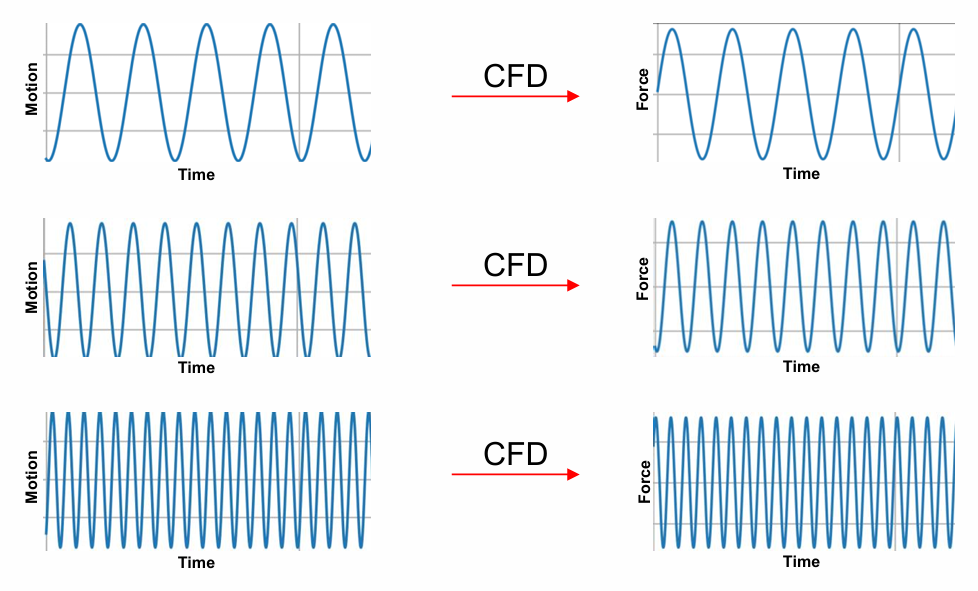
\includegraphics[width=1\textwidth]{Chap_1/Figures/Single_Frequency.png}
    \caption{Single Frequency Approach}
    \label{fig:Single_Frequency_Approach}
\end{figure}



\begin{figure}[htbp]
    \centering
    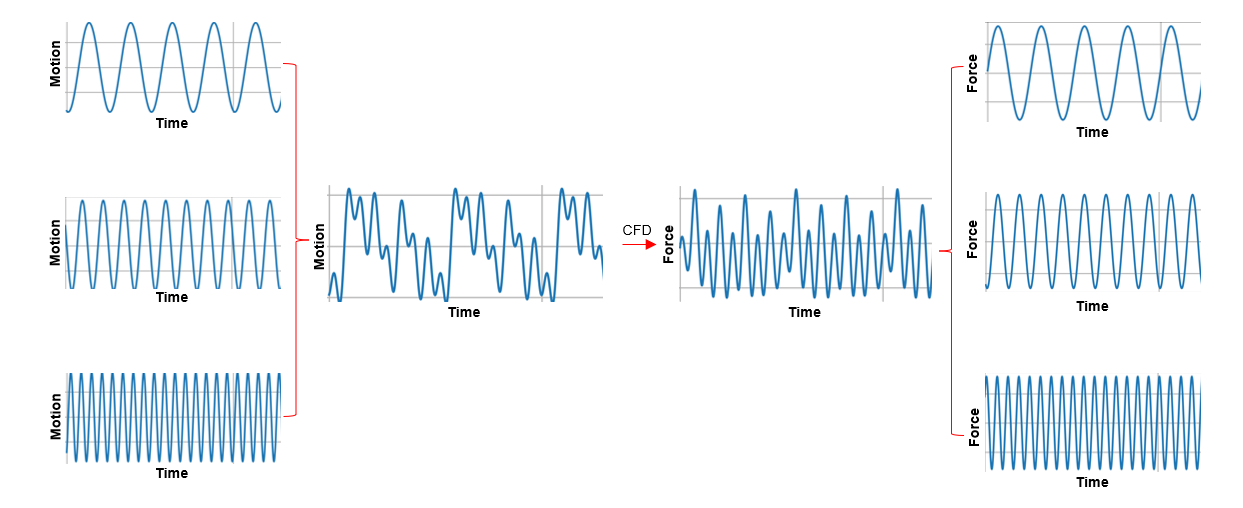
\includegraphics[angle=0, width=1.0\textwidth]{Chap_1/Figures/MultiFrequency_Explanation.png}
    \caption{Multi Frequency Approach}
    \label{fig:MultiFrequency_Approach}
\end{figure}
\newpage

%%%%%% Chap - 2 %%%%%%

\section*{Chapter 3:    Virtual Wind Tunnel Setup}

In this section, model setup for the virtual wind tunnel with CFD is described. The following are the tasks conducted\\ 

1. Creation of CFD model Geometry. \\
2. Specifying solver information for fluid and structural domain. \\
3. Finding the optimal mesh size for the Fluid domain with Mesh Convergence Study

\vspace{0.5 cm}

\subsection*{CFD Model:} 

The 2-D CFD model is created using GiD~\ref{fig:Virtual_Wind_Tunnel_Dimensions}. 
Since forced motion oscillation tests are conducted, the structure, ie the bridge 
deck cross-section is modelled as an opaque object in the fluid domain without any physics parameters 
like Stiffness and mass. Hence it is a one-way coupling. The bridge deck cross-section is taken from Sarkic
(Reference1), shown in Figure~\ref{fig:Sarkic_Section}. It is then externally oscillated by the solver with a 
specific frequency. Arbitrary Lagrangian-Eulerian (ALE) framework is used for this. \\

The Fluid domain is meshed with finer meshes near the structure and with coarser meshes farther away to have an optimal 
meshing. Hence, to produce smoother mesh transitions, fluid domain is divided into five subregions \ref{fig:GiD_Model_2}

\vspace{0.5 cm}

\begin{figure}[htbp]  
    \centering
    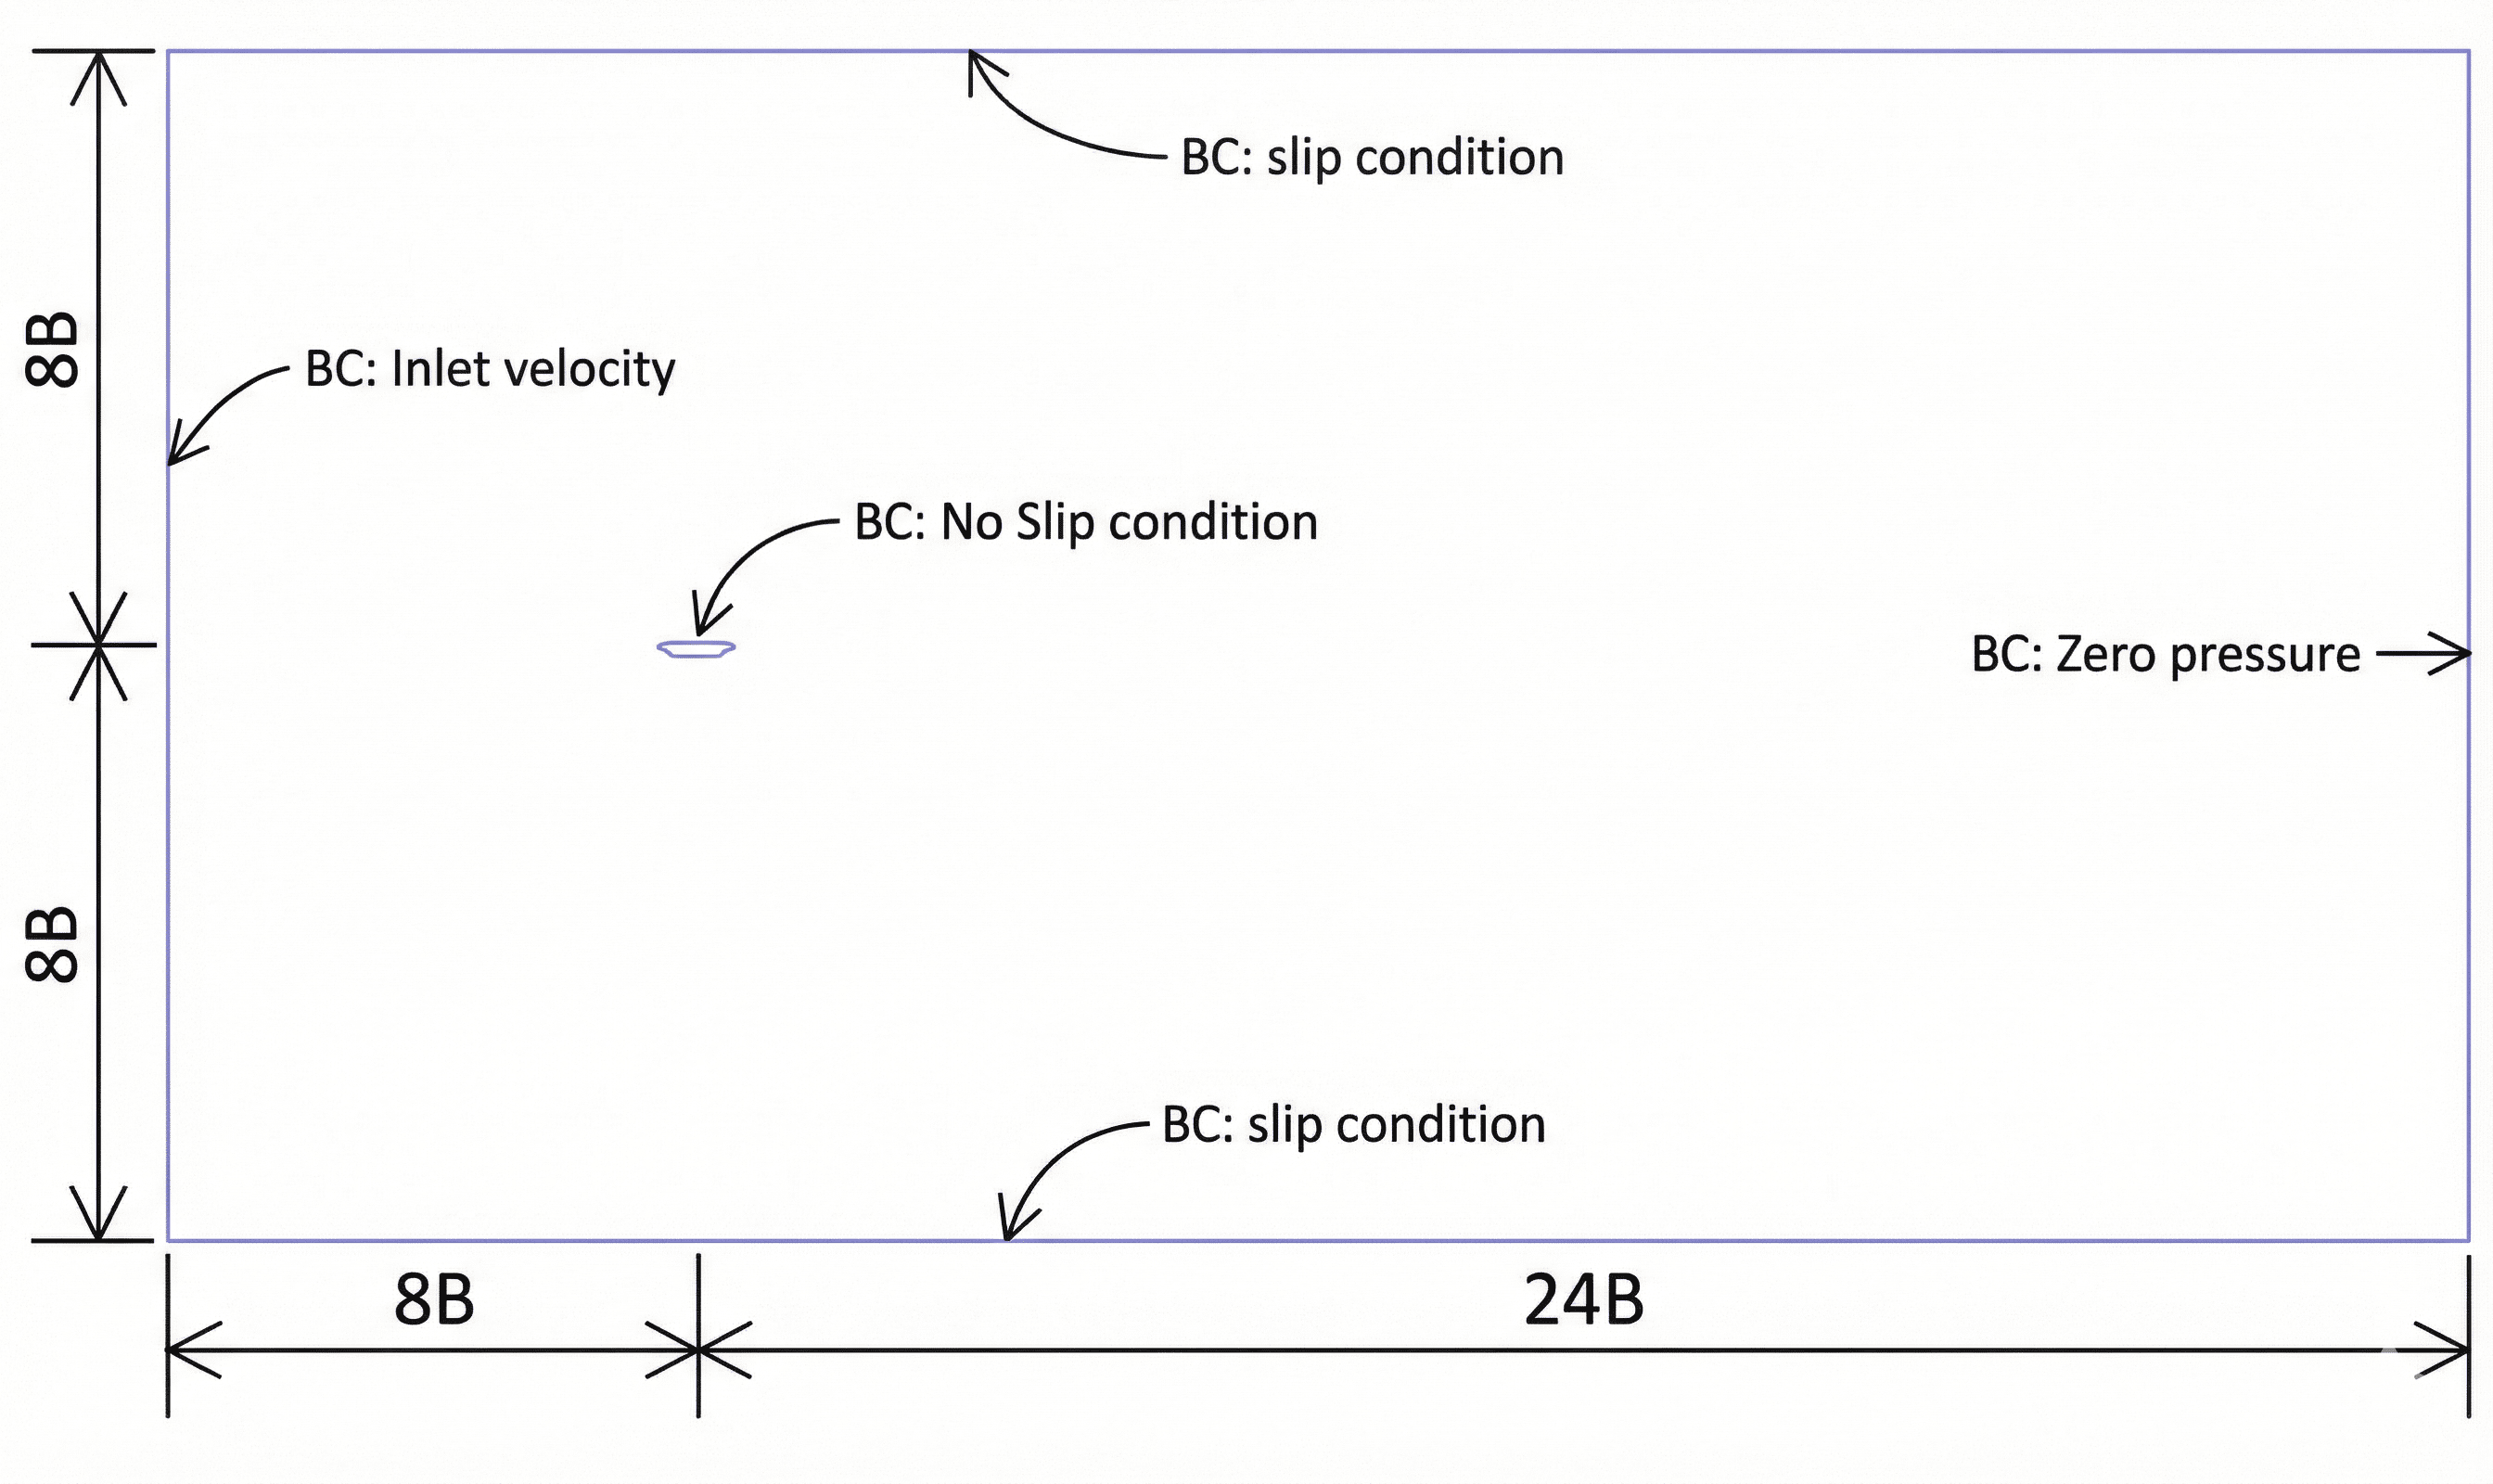
\includegraphics[width=0.65\textwidth]{Chap_2/Figures/Virtual_Wind_Tunnel_Dimensions.png}
    \caption{Virtual Wind Tunnel Dimensions}
    \label{fig:Virtual_Wind_Tunnel_Dimensions}
\end{figure}


\begin{figure}[htbp]  
    \centering
    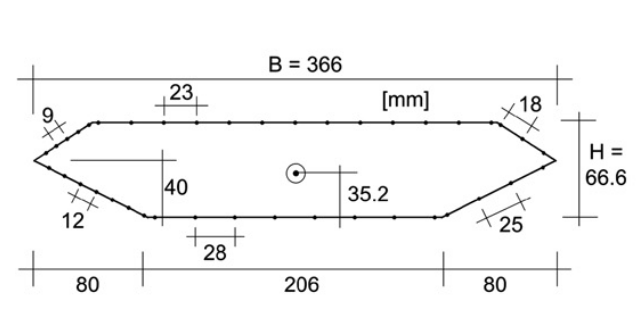
\includegraphics[width=0.5\textwidth]{Chap_2/Figures/Sarkic_Section.png}
    \caption{Sarkic Cross-Section}
    \label{fig:Sarkic_Section}
\end{figure}

\vspace{0.5 cm}

\subsection*{Solver Information:} 

The GiD model is solved with an open source Multiphysics solver - KratosMultiphysics. 
The boundary conditions applied to Fluid domain are shown in Figure~\ref{fig:Virtual_Wind_Tunnel_Dimensions}. 
The turbulence is modeled with URANS and the turbulence intensity is set to 0.1 and the turbulent mixing length is set to 0.0588 m.\\

The velocity is set to 1 m/s and the corresponding Reynolds number for the flow is $2.43*10^4$. The time step is 
taken as 0.002 seconds. The total simulation time can be divided into three phases: ramp-up time, stabilization time, and stable 
time period. In Ramp-up phase the flow velocity is steadily increased from 0 to 1 m/s to avoid numerical instabilities. 
In Stabilization phase, the flow is allowed to stabilize. The stable time period is the duration used for analysis. 
Ramp-up time and stabilization time are determined based on the vortex shedding frequency of the section.
From EN 1991, the Strouhal number of the section is taken as 0.1. \\ [0.1cm]

Vortex shedding frequency = $ \frac{0.1 * 1}{0.366} $ = 0.273 Hz \\ [0.1cm]
Ramp up time = $ 2 * \frac{1}{0.273} $ = 7.32 seconds \\ [0.1cm]
Stabilization time = $ 2 * \frac{1}{0.273} $ = 7.32 seconds \\ [0.1cm]

The stable time period is for capturing the flow behaviour. Since the interest of this thesis is to capture the flutter response, 
stable time period is time taken for 10 complete forced motion oscillations. But as each reduced velocity 
has a different forced motion frequency, the stable phase of the simulations is different. A higher reduced velocity will 
have a lower oscillating frequency and hence requiring a higher time of simulation and vice versa. Hence its calculation is 
shown after the information about the applied motion frequency is provided and in the consecutive chapters if any other 
reduced velocity is taken, the stable time period is mentioned in the respective chapter.

\begin{figure}[htbp]  
    \centering
    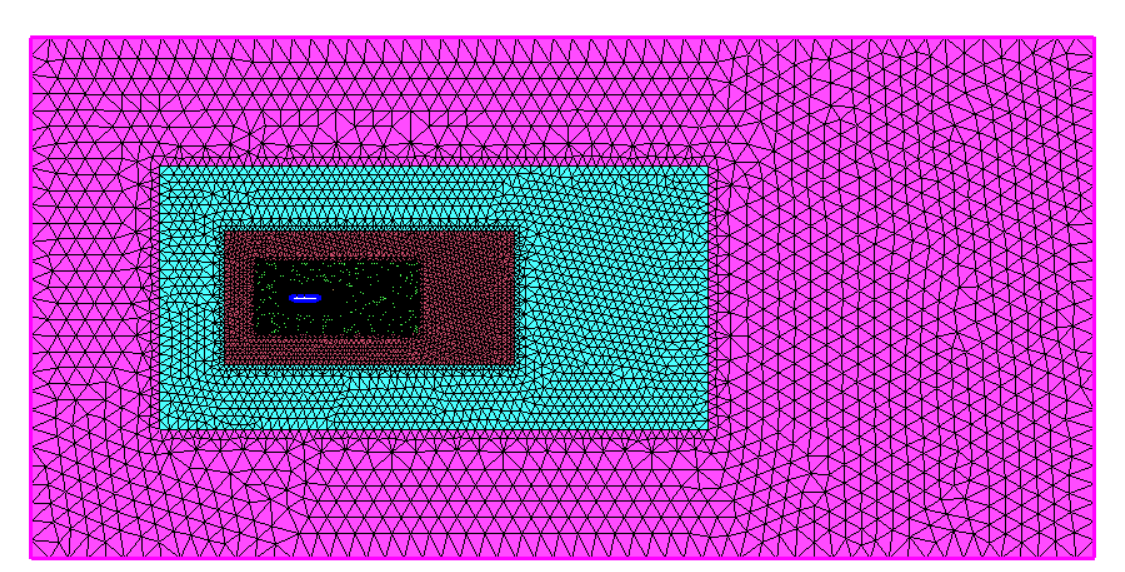
\includegraphics[width=0.65\textwidth]{Chap_2/Figures/GiD_Model_2.png}
    \caption{GiD Model of Virtual Wind Tunnel}
    \label{fig:GiD_Model_2}
\end{figure}

\vspace{0.5 cm}

\subsection*{Mesh Convergence Study:} 

A mesh convergence study is conducted to determine the optimal mesh element size. Five models with progressive 
mesh sizes are created and convergence of 8 derivatives are analysed. The Table~\ref{tab:mesh_convergence} shows the models
and corresponding mesh sizes at each zone. The study is performed for a single point on the flutter derivative curve
at a reduced velocity of 10.93. From the literature review, it is identified 5$\%$ of width of bridge deck as the heave amplitude 
and 5 degree as pitch amplitude are the appropriate forced motion amplitude such that aerodynamic forces show linear behaviour.  \\ [0.1cm]

Heave amplitude = $ \frac{5 * 0.366}{100} $ = 0.0183 m\\ [0.1cm]
Pitch amplitude = 0.087 radians\\ [0.1cm]
Motion Frequency = 0.25 Hz\\ [0.1cm] 
Stable time period = $ 10 * \frac{1}{0.25} $ = 40 seconds\\ [0.1cm]
Total simulation time = Ramp-up time + Stabilization time + Stable time period = 7.32 + 7.32 + 40 = 54.64 seconds\\ [0.1cm]


\begin{table}[htbp]  
    \centering
    \caption{Mesh Convergence Study Results}
    \label{tab:mesh_convergence}
    \begin{tabular}{|l|c|c|c|c|c|}
        \hline
        \textbf{} & \textbf{Model 1} & \textbf{Model 2} & \textbf{Model 3} & \textbf{Model 4} & \textbf{Model 5} \\ \hline
        Zone A (m) & 0.25 & 0.25 & 0.2304 & 0.2112 & 0.192 \\ \hline
        Zone B (m) & 0.1 & 0.12 & 0.1152 & 0.1056 & 0.096 \\ \hline
        Zone C (m) & 0.054 & 0.08 & 0.0576 & 0.0528 & 0.048 \\ \hline
        Zone D (m) & 0.018 & 0.025 & 0.0288 & 0.0264 & 0.024 \\ \hline
        Zone E (m) & - & - & 0.0096 & 0.0088 & 0.008 \\ \hline
        Zone F (m) & 0.009 & 0.008 & 0.0048 & 0.0044 & 0.004 \\ \hline
        Deck Surface (m) & 0.0045 & 0.003 & 0.0024 & 0.0022 & 0.002 \\ \hline
        Width/ min mesh size & 81.333 & 122 & 152.5 & 166.36 & 183 \\ \hline
        Total Elements & 7368 & 15704 & 20854 & 24374 & 29408 \\ \hline
        Minimum Mesh Size GID & 0.00358 & 0.00245 & 0.00196 & 0.00179 & 0.00159 \\ \hline
        Velocity (m/s) & 1 & 1 & 1 & 1 & 1 \\ \hline
        Time step & 0.004 & 0.002 & 0.002 & 0.002 & 0.002 \\ \hline
        CFL & 1.11 & 0.81 & 1.02 & 1.11 & 1.26 \\ \hline
    \end{tabular}
\end{table}

With this simulation setup, the CFD simulations are conducted for all five models figure~\ref{fig:CFD_Result}. 
This magnitude of heave and pitch amplitudes are applied and corresponding aerodynamic lift and moment
forces are identified. The aerodynamic forces are then used to calculate the flutter derivatives. The convergence of flutter derivatives is then analysed. 
Figure~\ref{fig:Heave_Motion} shows the aerodynamic lift and moment forces obtained for Model 3. 


\begin{figure}[htbp]  
    \centering
    
\includegraphics[width=0.65\textwidth]{Chap_2/Figures/CFD_Result.png}
    \caption{CFD Results for Model 3}
    \label{fig:CFD_Result}
\end{figure}

\vspace{0.5 cm}

\begin{figure}[htbp]
    \centering
    \begin{subfigure}{\textwidth}
        \centering
        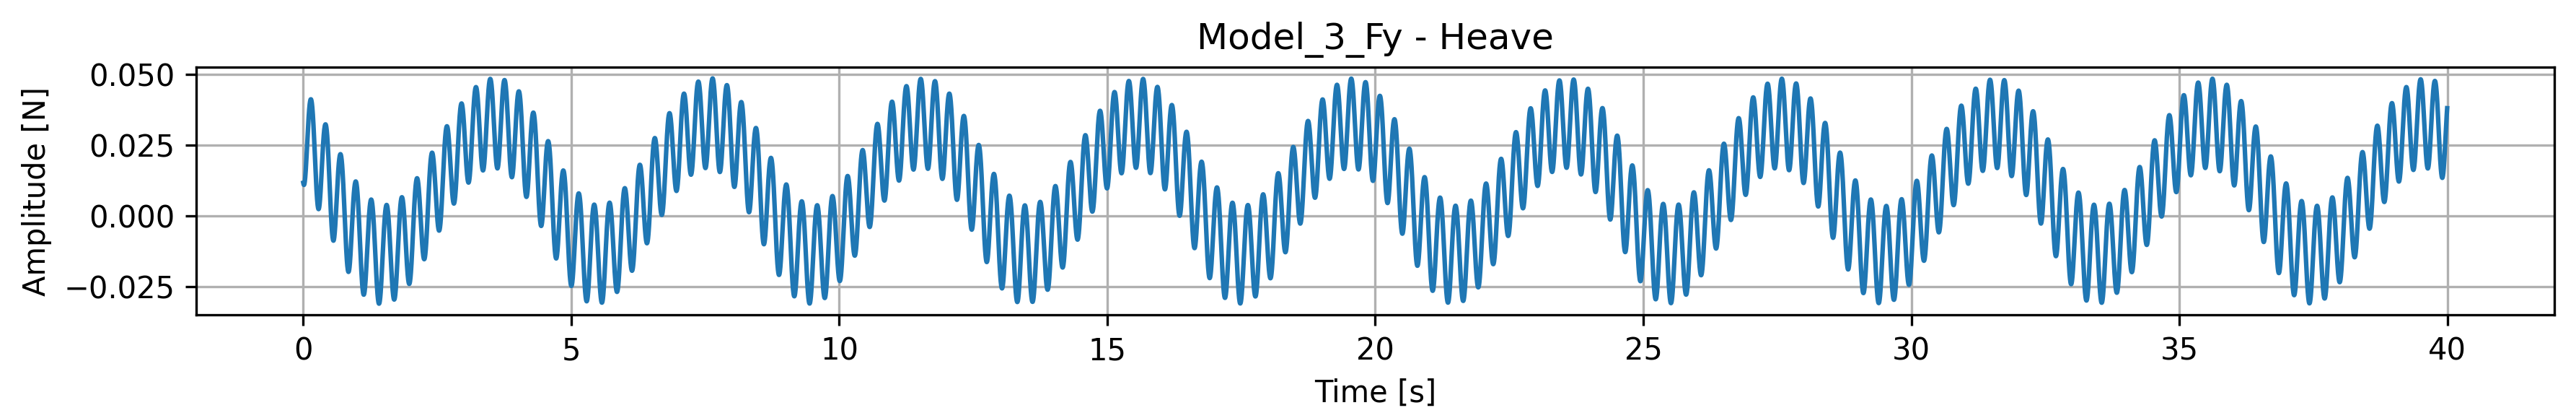
\includegraphics[width=1\textwidth]{Chap_2/Figures/Model_3_Fy_and_Components_Heave.png}
        \caption{$F_y$}
        \label{fig:Model_3_Fy_Heave}
    \end{subfigure}
    \vspace{0.5cm}
    \begin{subfigure}{\textwidth}
        \centering
        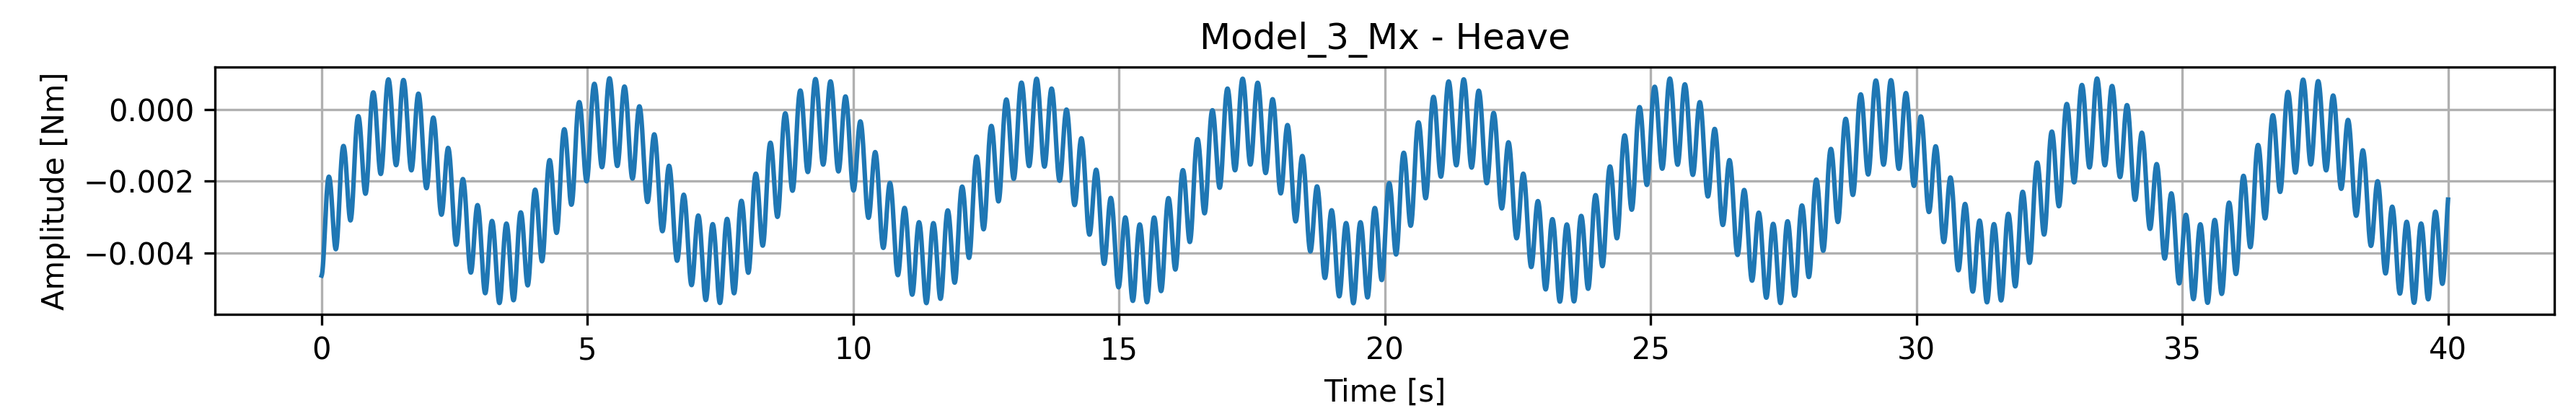
\includegraphics[width=1\textwidth]{Chap_2/Figures/Model_3_Mx_and_Components_Heave.png}
        \caption{$M_x$}
        \label{fig:Model_3_Mx_Heave}
    \end{subfigure}
    \caption{Heave Motion}
    \label{fig:Heave_Motion}
\end{figure}

The results of the mesh convergence study are shown in Figure~\ref{fig:convergence}. It is observed that the 
derivatives $H_1,H_3,A_1,A_2,$ and $A_3$ exhibited good convergence, while derivatives  $H_2,H_4,$ and $A_4$ displayed 
oscillatory convergence behavior. This behavior is consistent with findings in the literature, as these 
particular derivatives are known to be more difficult to capture accurately. From the study it is concluded, 
Model 3 is optimal and this mesh size is used for all subsequent simulations.

%% Figures for Mesh Convergence Study
\begin{figure}[htbp]  
    \centering
    \begin{subfigure}[b]{0.45\textwidth}
        \centering
        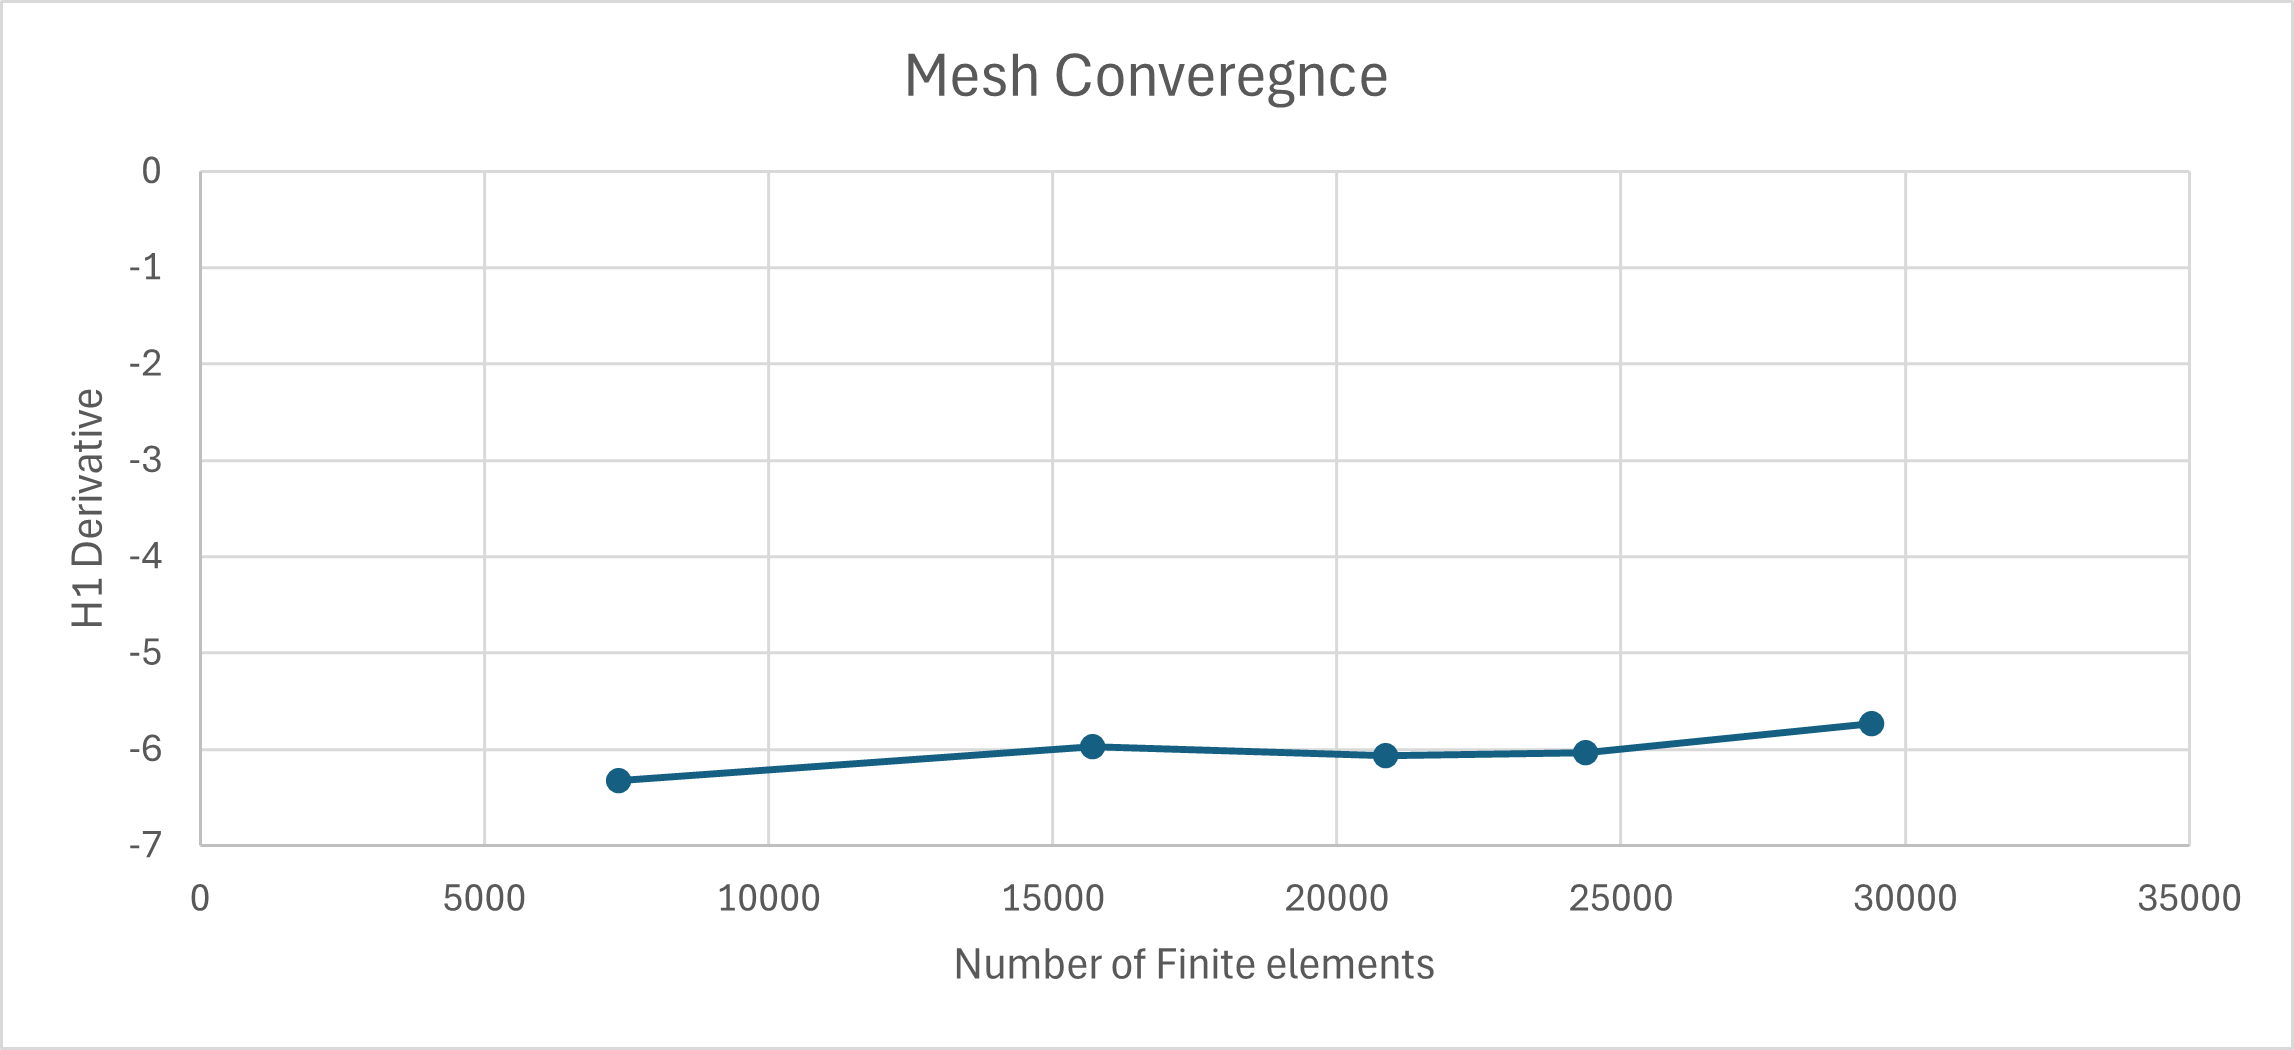
\includegraphics[width=\textwidth]{Chap_2/Figures/Convergence_Study_H1}
        \caption{H1}
        \label{fig:h1}
    \end{subfigure}
    \hfill
    \begin{subfigure}[b]{0.45\textwidth}
        \centering
        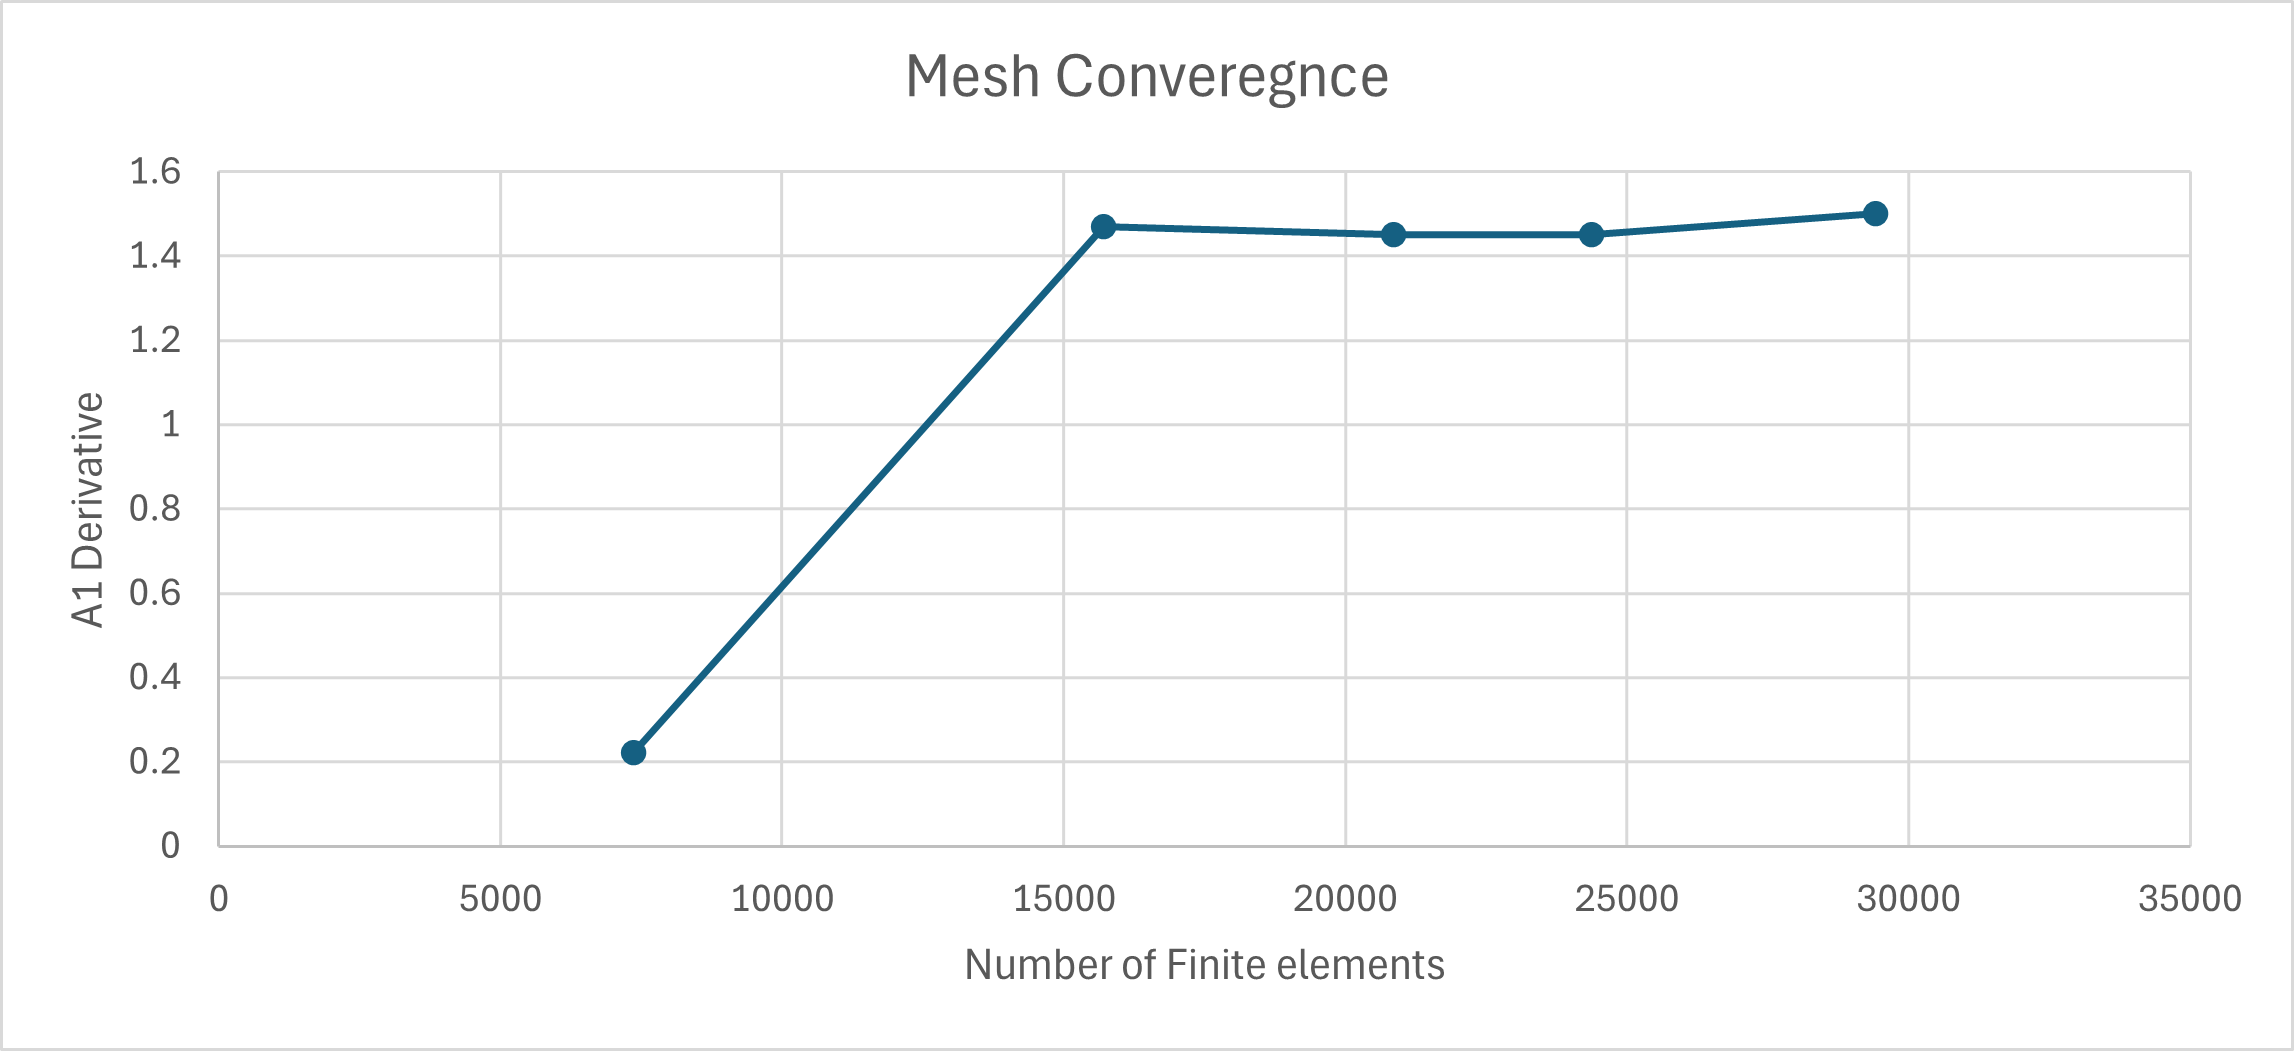
\includegraphics[width=\textwidth]{Chap_2/Figures/Convergence_Study_A1}
        \caption{A1}
        \label{fig:a1}
    \end{subfigure}
    
    \begin{subfigure}[b]{0.45\textwidth}
        \centering
        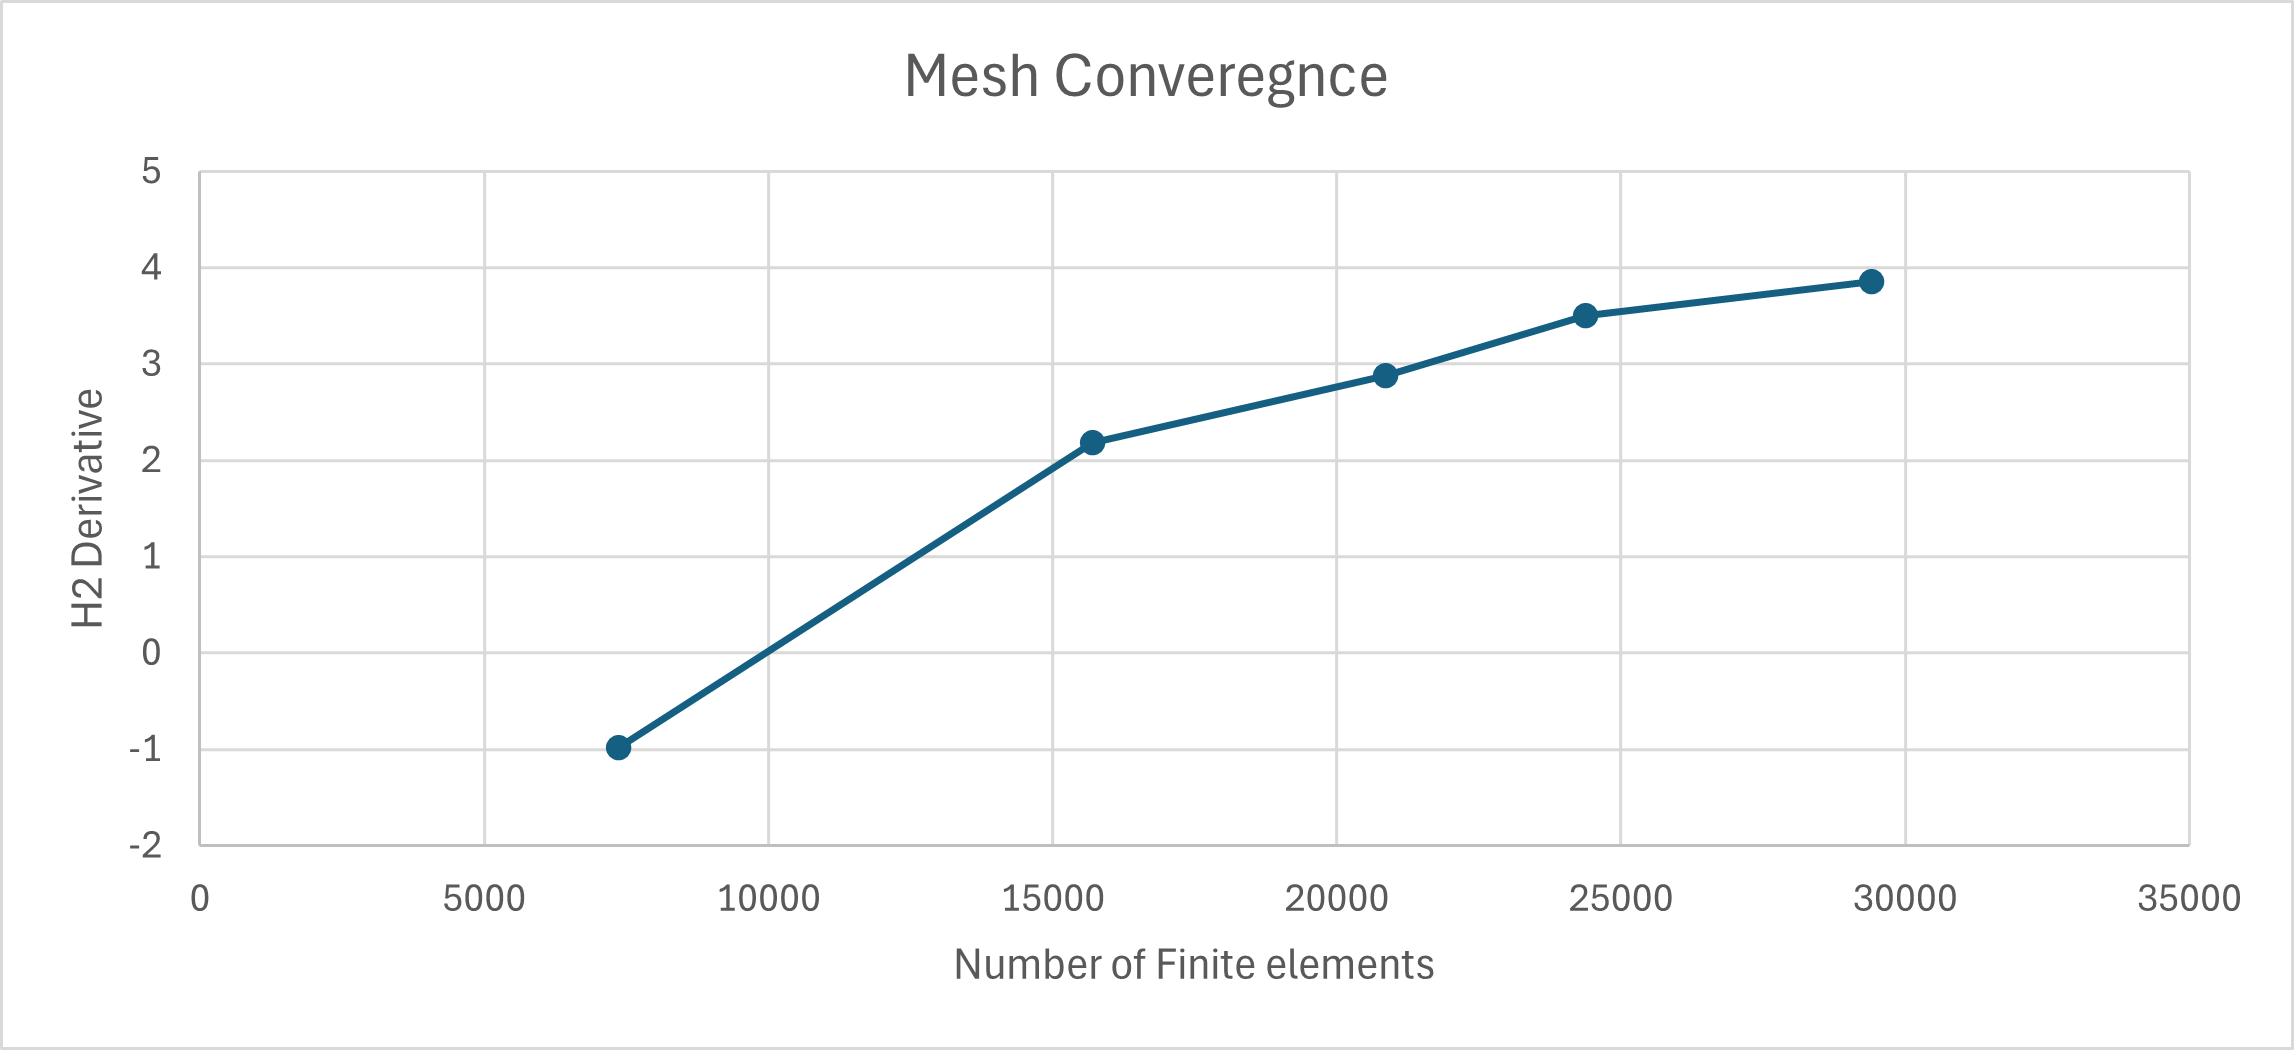
\includegraphics[width=\textwidth]{Chap_2/Figures/Convergence_Study_H2}
        \caption{H2}
        \label{fig:h2}
    \end{subfigure}
    \hfill
    \begin{subfigure}[b]{0.45\textwidth}
        \centering
        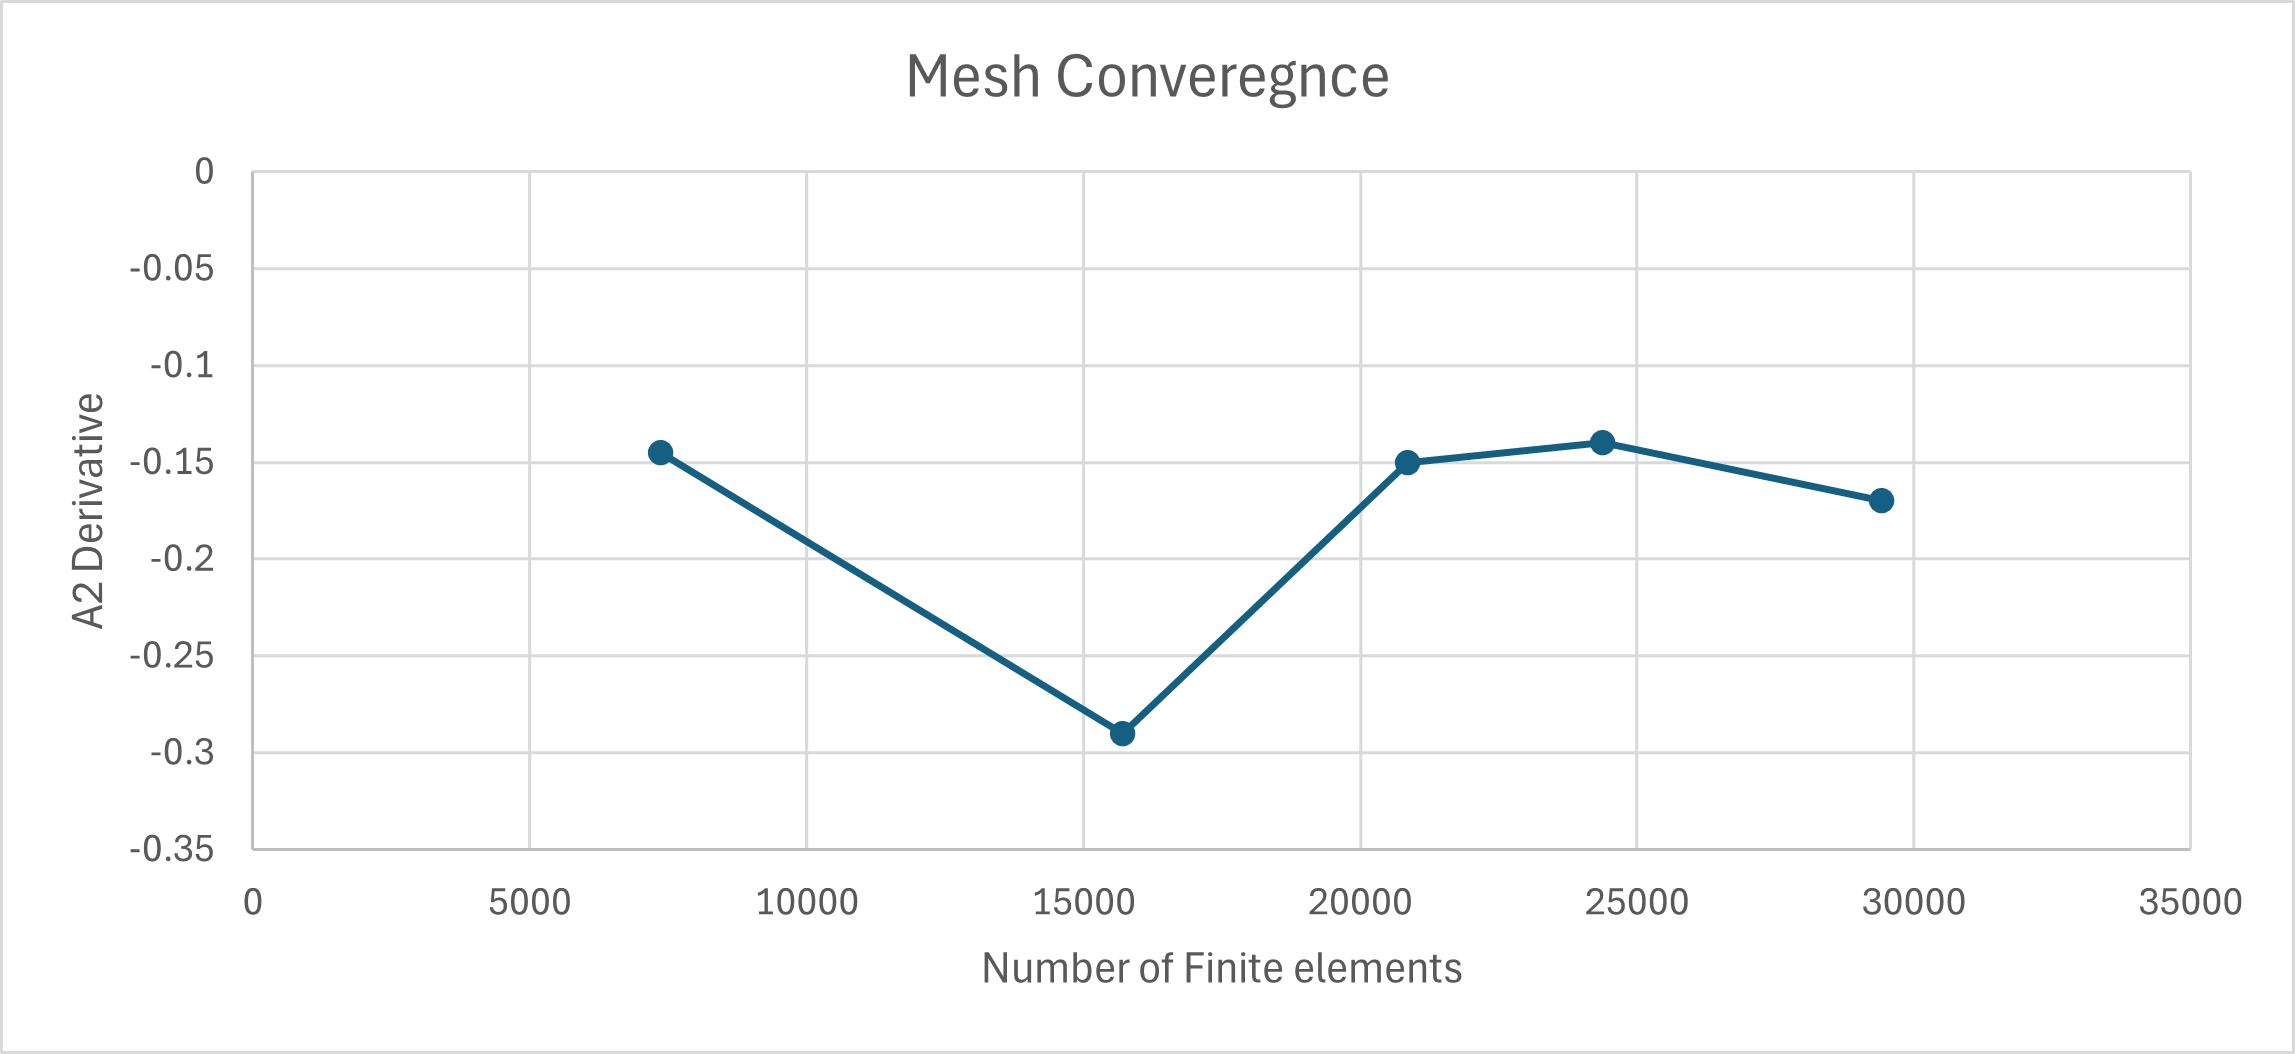
\includegraphics[width=\textwidth]{Chap_2/Figures/Convergence_Study_A2}
        \caption{A2}
        \label{fig:a2}
    \end{subfigure}
    
    \begin{subfigure}[b]{0.45\textwidth}
        \centering
        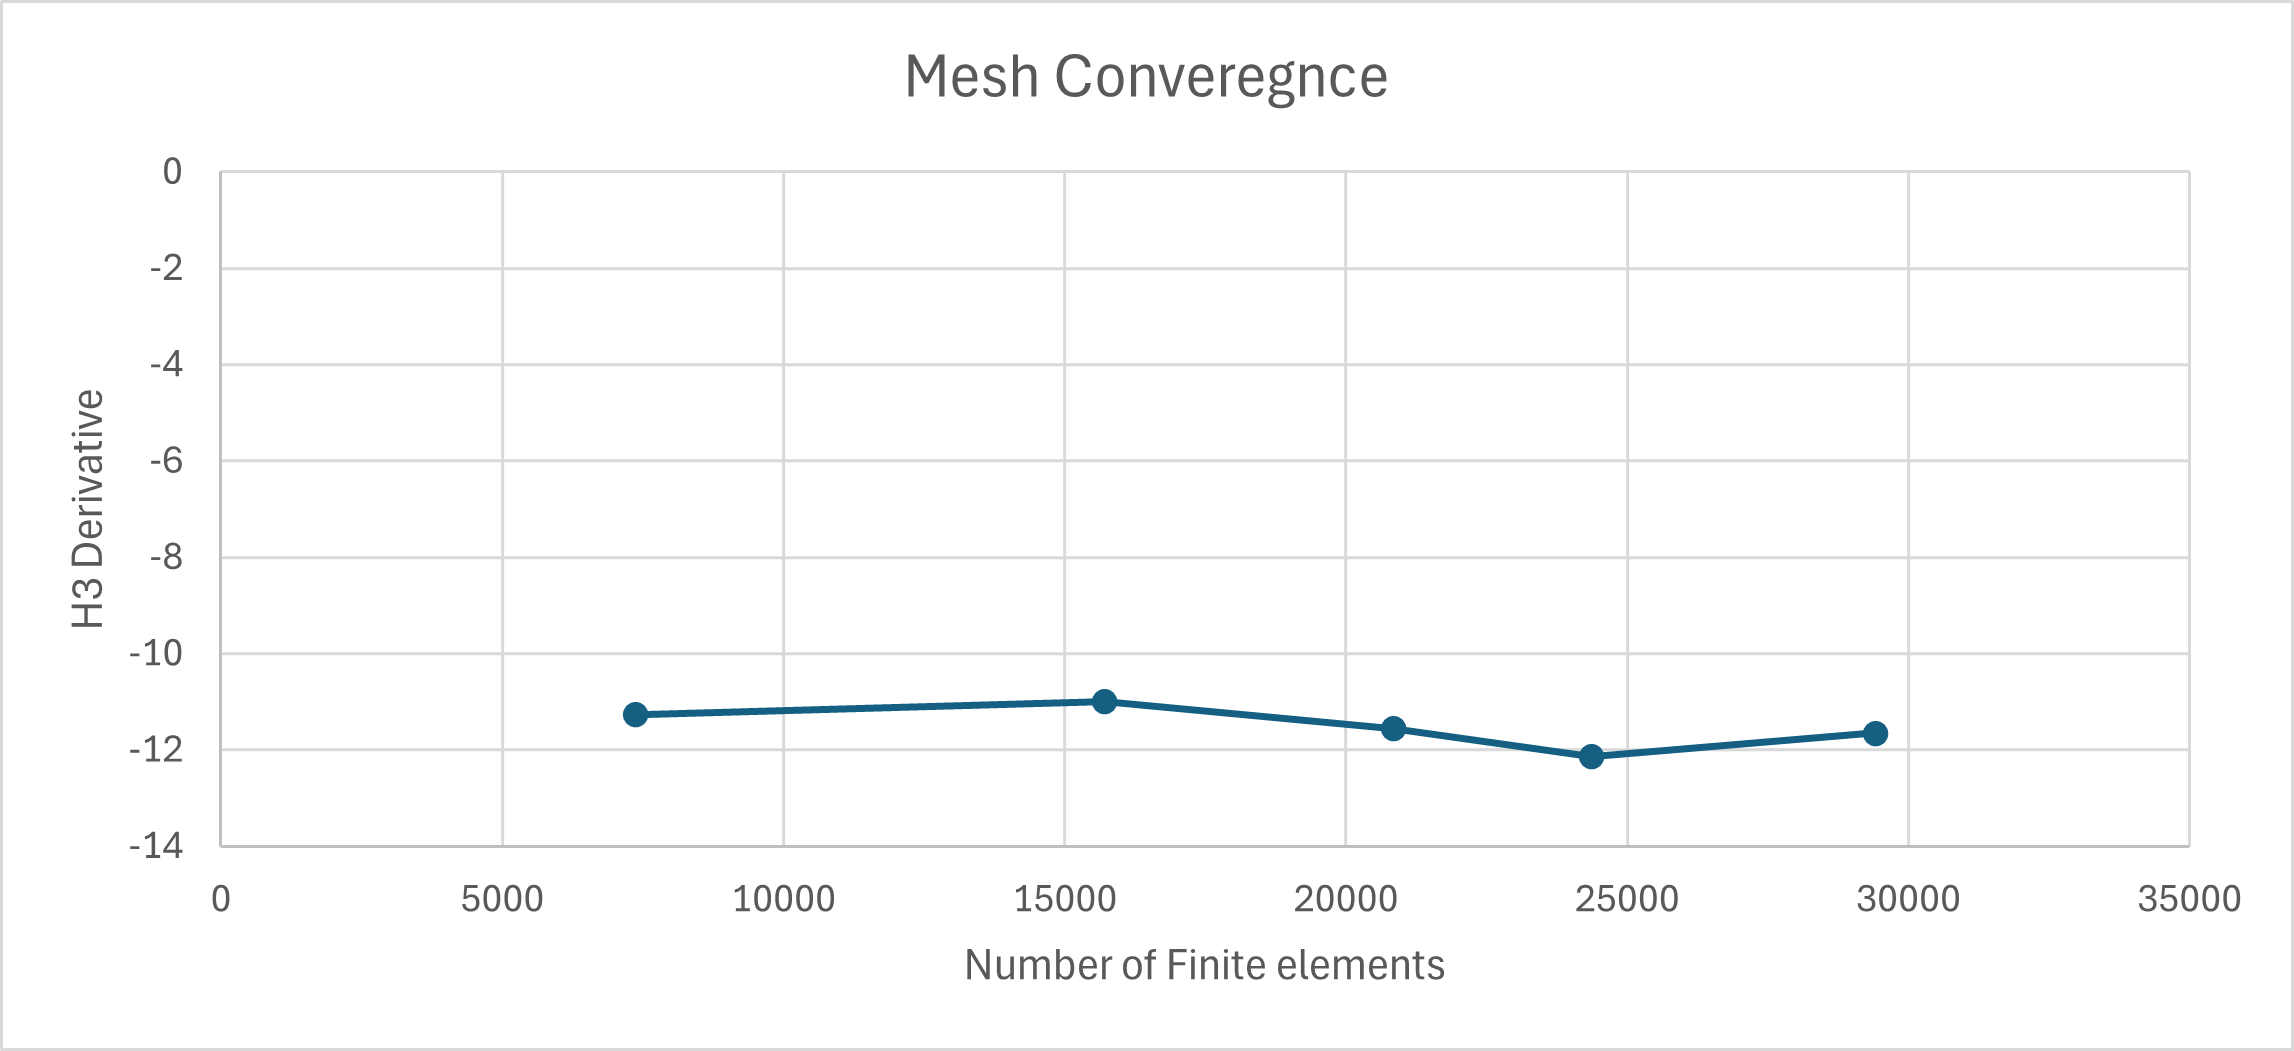
\includegraphics[width=\textwidth]{Chap_2/Figures/Convergence_Study_H3}
        \caption{H3}
        \label{fig:h3}
    \end{subfigure}
    \hfill
    \begin{subfigure}[b]{0.45\textwidth}
        \centering
        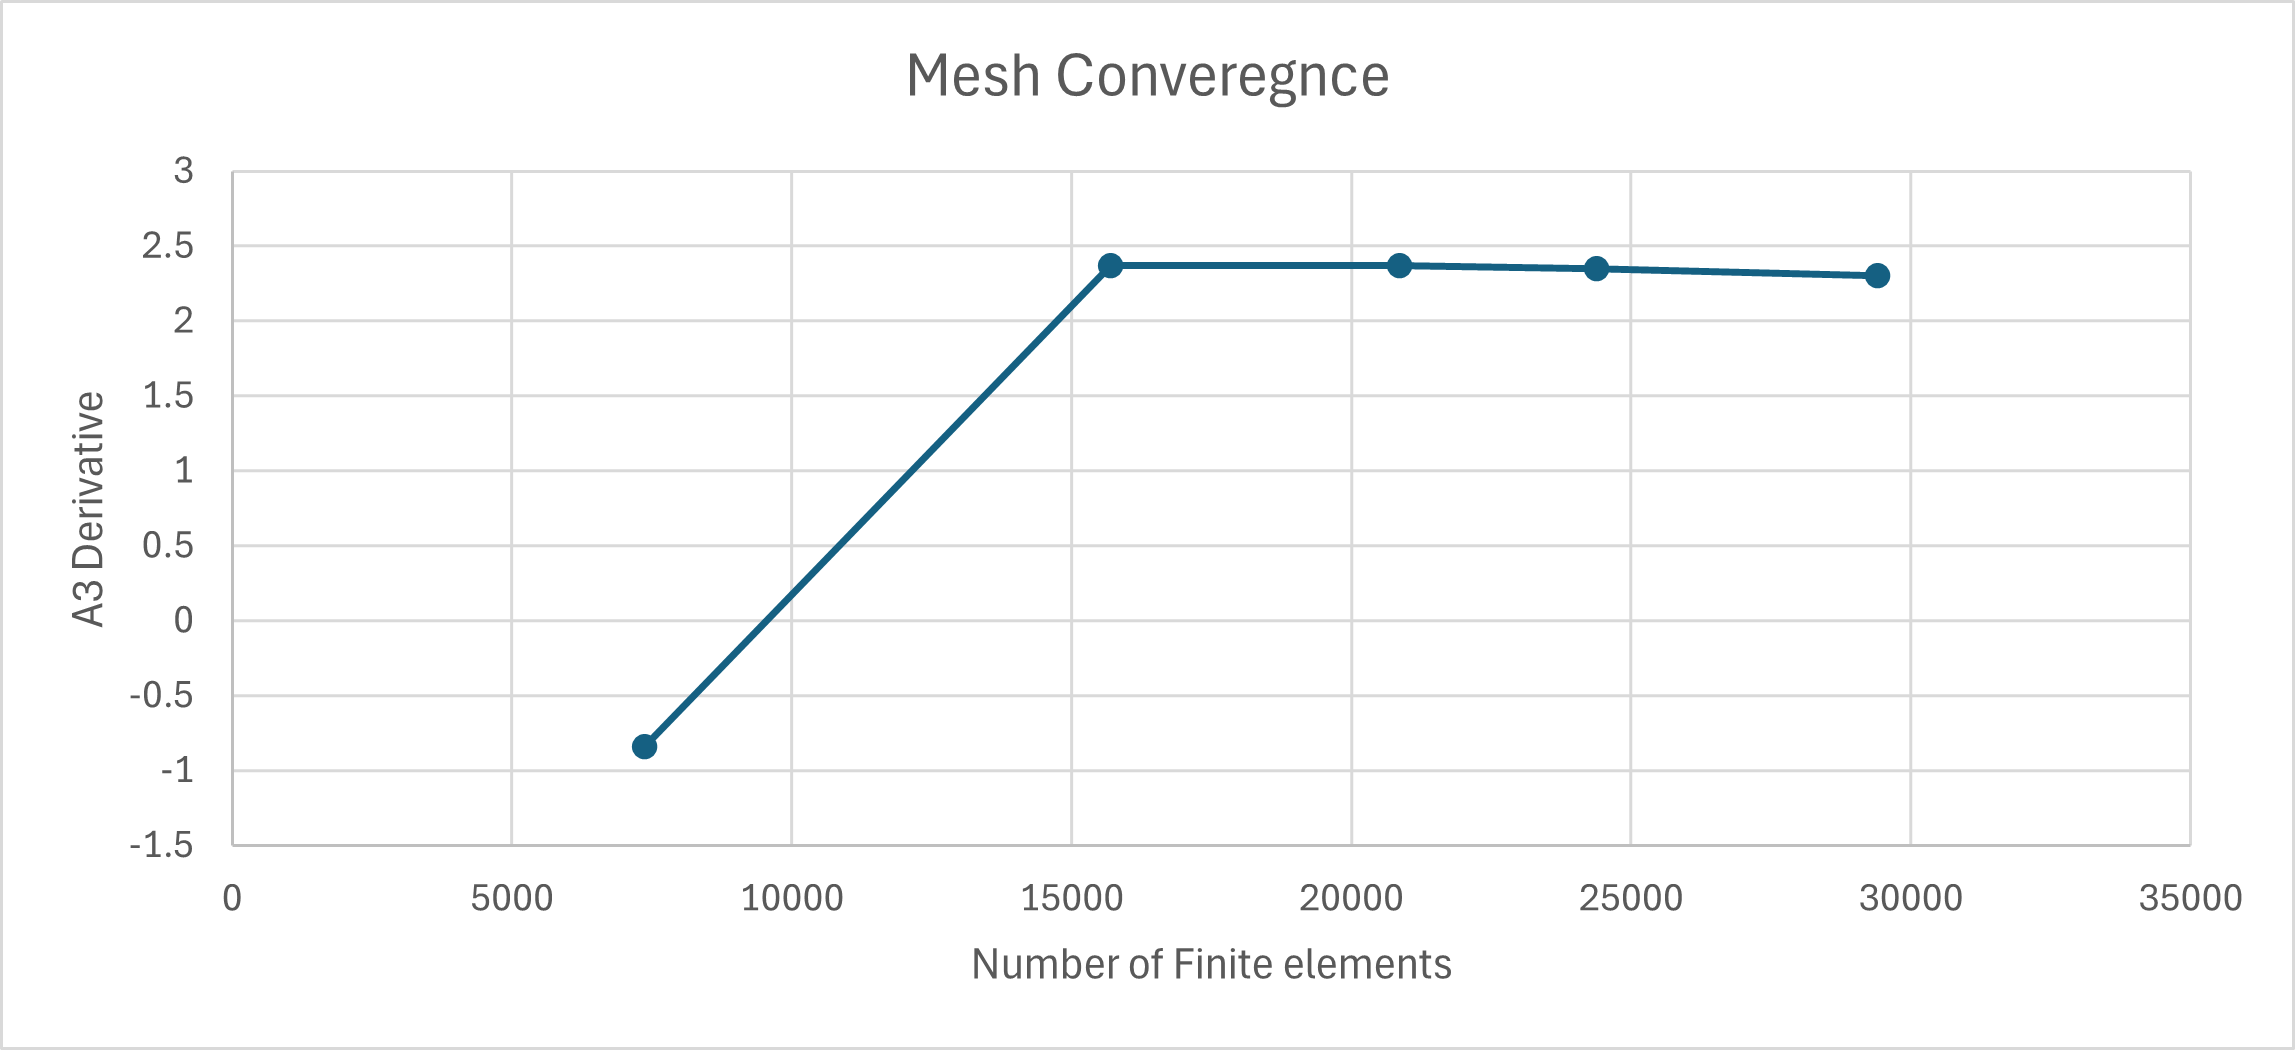
\includegraphics[width=\textwidth]{Chap_2/Figures/Convergence_Study_A3}
        \caption{A3}
        \label{fig:a3}
    \end{subfigure}
    
    \begin{subfigure}[b]{0.45\textwidth}
        \centering
        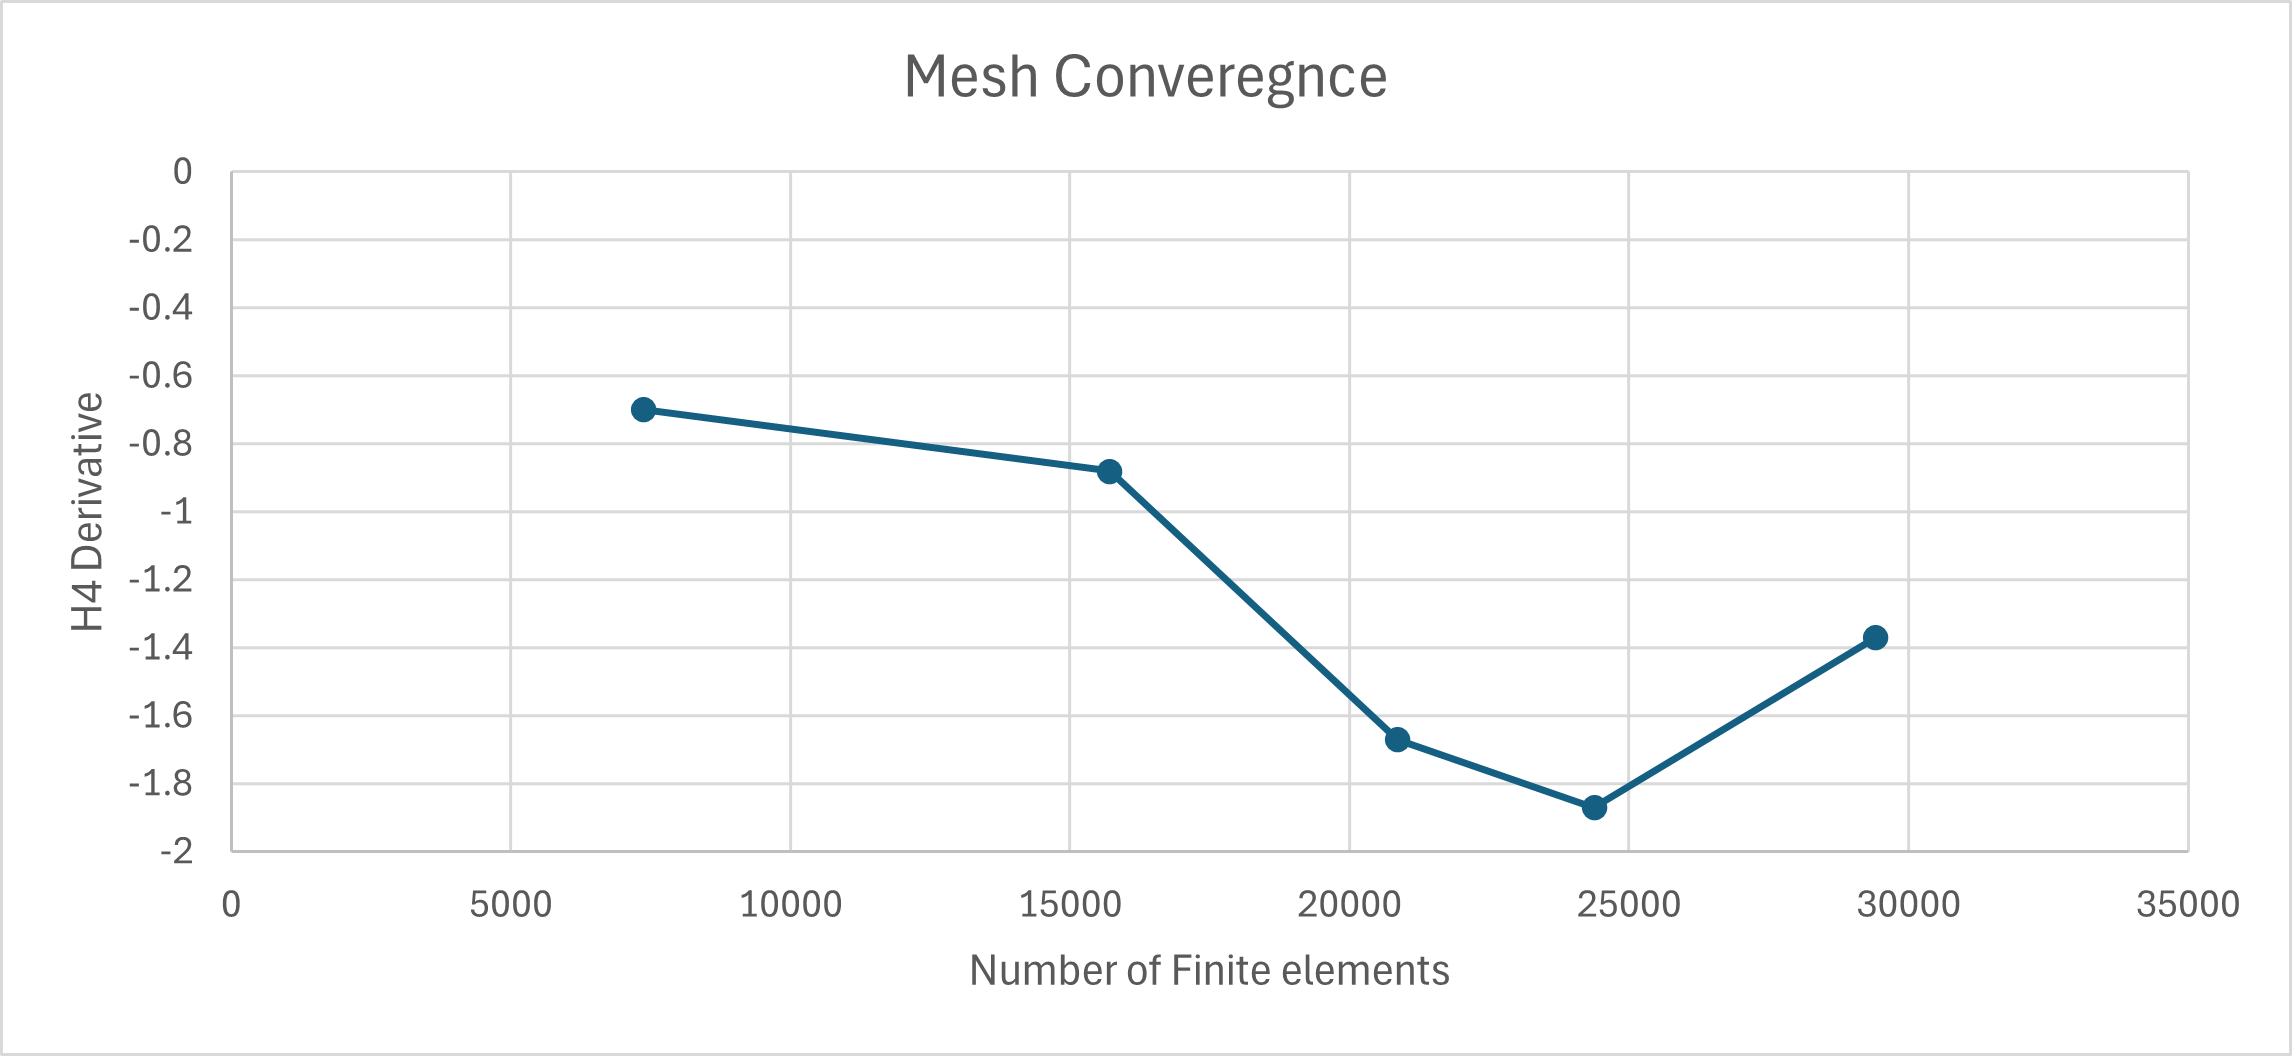
\includegraphics[width=\textwidth]{Chap_2/Figures/Convergence_Study_H4}
        \caption{H4}
        \label{fig:h4}
    \end{subfigure}
    \hfill
    \begin{subfigure}[b]{0.45\textwidth}
        \centering
        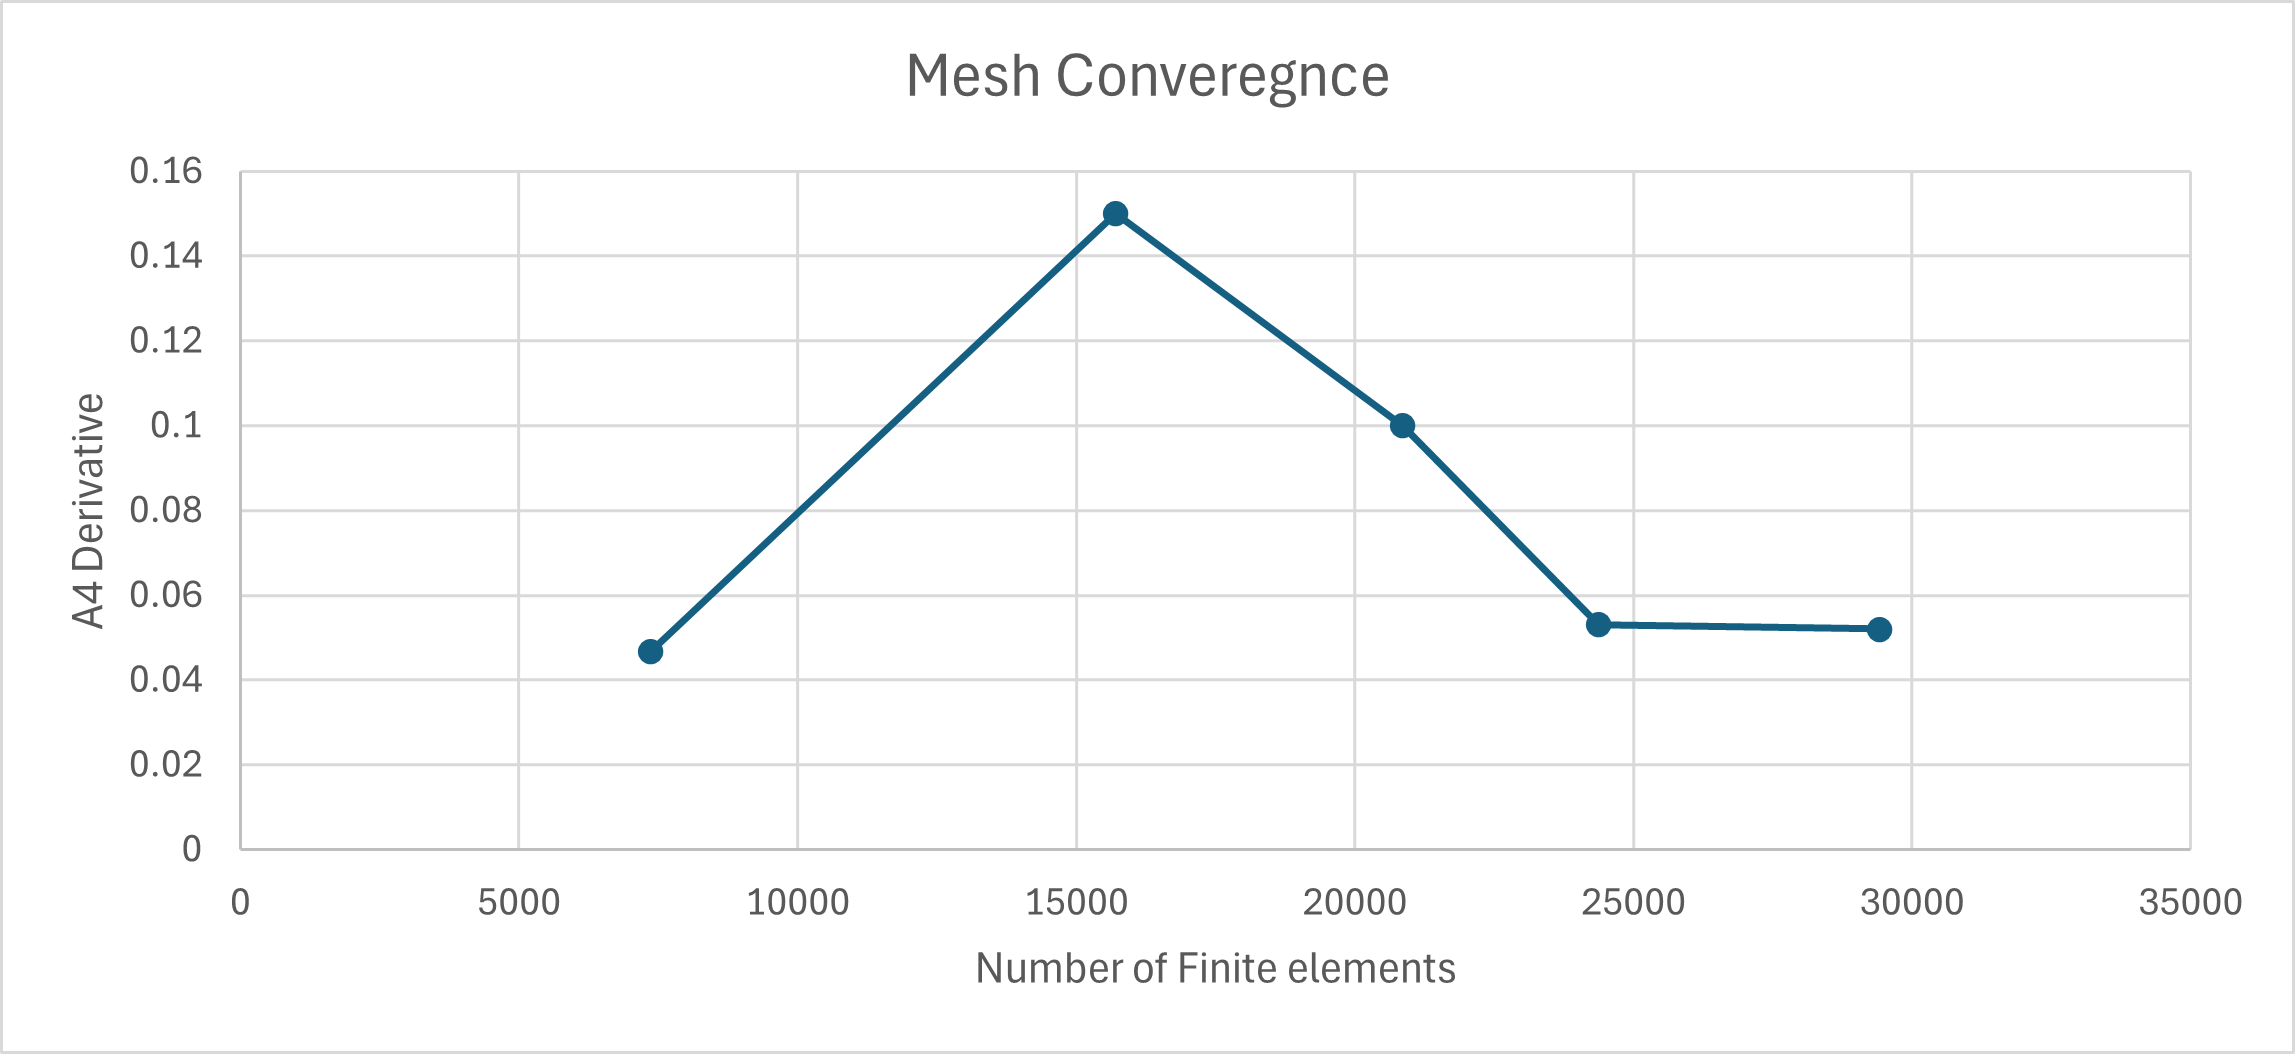
\includegraphics[width=\textwidth]{Chap_2/Figures/Convergence_Study_A4}
        \caption{A4}
        \label{fig:a4}
    \end{subfigure}
    
    \caption{Mesh Convergence Study Results}
    \label{fig:convergence}
\end{figure}

\end{document}